% Do not change the options here
\documentclass[bsc,frontabs,singlespacing,parskip,deptreport]{infthesis}

\usepackage{eushield}
\usepackage{hyperref, csquotes}
\usepackage{graphicx}
\usepackage{booktabs, multirow}
\usepackage[font={footnotesize,serif}]{caption}

\graphicspath{ {./figures/} }

\begin{document}
\begin{preliminary}

\title{Adaptable Multicore Processing in a Research Operating System}

\author{Kimberley \\ Elizabeth Stonehouse}

\course{Computer Science}

\project{4th Year Project Report}

\date{\today}

\abstract{
Multicore architectures are pervasive within the computing industry, demanding that computer science students master a thorough understanding of the underlying theoretical concepts. However, while the open-source nature of prominent operating systems such as Linux offers the potential for students to learn about the internals of real operating systems, the complexity of the codebases make them extremely difficult to understand, particularly for novice programmers. Furthermore, the intricacy of such operating systems makes experimenting with new performance improvements almost impossible without introducing difficult-to-detect bugs. This project solves both of these problems by adding multicore processing support to a research operating system, InfOS. By redesigning InfOS specifically with multiple cores in mind, we produce a well-structured, modular implementation that can be used as a valuable teaching tool to help undergraduate students grasp multicore concepts. Furthermore, we produce a research platform for investigating intelligent scheduling approaches, and discuss how this platform will be used for a future research paper on cache-aware scheduling.
}

\maketitle

\section*{Acknowledgements}
I owe my achievements to a great many people.

To my supervisor, Dr Tom Spink, for his unparalleled and tireless support throughout this entire project, particularly when the cores were misbehaving. Additionally, for his enthusiasm for systems research that inspired me to pursue a PhD.

To my truly incredible friends Jen and George, who have provided unwavering support throughout some very challenging times. It most certainly would not have been possible without you.

To my wonderful flatmates, Sarah and Orlagh, for being an endless source of laughter. Your constant positivity and enthusiasm motivates me.

Lastly, to my family, for their continuous support during my four years at university and their encouragement to continue to postgraduate study.

\tableofcontents
\end{preliminary}

\chapter{Introduction}
For decades, Moore’s law scaling has predicted exponential advancements in computing performance. However, with Moore’s law coming to an end and power consumption becoming an increasingly constraining factor, chip makers have turned to multicore architectures. A multicore processor has two or more processing units, or cores, on the same chip, and can provide performance improvements without unsustainable power consumption. In 2001, IBM released the POWER4, the industry’s first server chip with two cores \cite{power4}, then in 2005 came the Athlon 64 X2, AMD’s first desktop dual-core processor. Today, the multicore trend shows no signs of slowing down. The Sunway TaihuLight supercomputer has 256 cores per processor chip, amounting to over 10 million cores across the entire system \cite{sunway}. With multicore architectures being so pervasive in computing, it is especially important for students to develop a good understanding before entering the industry. However, multicore concepts are not easy to grasp, and parallel programming is particularly challenging. Expert programmers must explicitly divide tasks into threads that can be run concurrently, and avoid synchronisation issues while doing so \cite{geer}. 

It is possible for the operating system to simplify the programmer's task by presenting a clean, well-structured, multicore interface; however, most operating systems do not. In fact, most modern operating systems are extremely complex and difficult to understand. For example, the Linux kernel has evolved over a period of thirty years into a project comprising over 27.8 million lines of code \cite{linux-loc} with around six thousand developers \cite{linux-kernel}. While the open-source nature of Linux makes it a good educational resource, with all source code being publicly available on GitHub \cite{linux-github}, the large and unwieldy nature of the project makes it almost impossible for a novice programmer to understand. The code is not particularly readable, and demands a good mastery of low-level technical concepts such as pointers. In essence, while being a freely-accessible example of an established operating system, Linux is not particularly useful as a teaching tool. 

Furthermore, as researchers continue searching for performance improvements, new scheduling policies have been developed that utilise system resources more efficiently \cite{wasted-cores}. However, the extensibility of traditional monolithic operating systems is limited, meaning that these policies rarely make their way into production operating systems. One study proposed that a modular scheduler could offer a solution, combining a multitude of factors such as resource contention, cache usage and workload balancing among cores. However, once an operating system is established, a modular redesign is not a feasible option. As an illustrative example, the cost of redeveloping Linux was estimated in 2011 at \$3 billion USD \cite{linux-kernel-cost}, and again in 2018 at \$14.7 billion USD \cite{cost-to-redev}. 

InfOS \cite{infos} is a research operating system that can provide a solution. InfOS was written entirely from scratch in C++ following an object-oriented design, and was developed precisely because modern operating system kernels like Linux are extremely complex. InfOS is a valuable teaching tool that is used to help undergraduate students to develop their understanding of operating system internals. InfOS currently only supports unicore processing, but being relatively lightweight in comparison to large-scale and long-lived operating systems, InfOS presents a rare opportunity to redesign an operating system specifically with multicore processing in mind. The object-oriented design of InfOS will extend naturally to support multicore processing in a well-structured manner, and adding this support will develop InfOS further as a teaching tool. This can also provide research advantages, since the scheduler can be designed in a modular way that allows experimenting with new scheduling policies easily. This project makes the following key contributions:

\begin{enumerate}
    \item A well-designed, object-oriented multicore operating system that can be easily understood by students.
    \item A working operating system implementation that can be downloaded and booted on real hardware by anyone.
    \item A platform on which to build further research and experiment with performance optimisations.
\end{enumerate}

\chapter{Background}
\section{Unicore Limitations} \label{unicore-limitations}
Moore’s Law predicts that the number of transistors per integrated circuit doubles roughly every two years \cite{moore_1998, moore_2006}. For decades, Moore’s Law scaling has correctly predicted exponential advancements in computing performance, which has set a precedent. However, this doubling cannot go on forever, and Moore’s law is coming to an end \cite{DBLP:journals/cse/TheisW17}. Still, our expectations have been set, and so the computing industry has begun to look to new ways of improving computing performance. This has ultimately introduced two key issues.

\subsection{The Power Wall} \label{the-power-wall}
In a processor, the operations performed are governed by a system clock, with each operation beginning on a pulse of the clock. These operations may include fetching an instruction, decoding an instruction or performing an arithmetic operation. It follows that fundamentally, the speed of the processor is determined by the speed of the clock, so chip manufacturers have historically improved performance by increasing the clock speed \cite{stallings}. The increased clock speed was achieved by shrinking the transistors, since smaller transistors can switch faster. Dennard scaling \cite{dennard_1999} suggested that as transistors shrank, their power density stayed constant, meaning that a chip's power use should stay proportional to its area. This should have allowed circuits to operate at higher frequencies without an increased power usage. However, this scaling rule ignored transistor leakage, which aggregates with a growing number of increasingly small transistors and drives up power consumption \cite{bohr_2007}.

This breakdown of Dennard scaling meant that increasing the clock speed demanded an increase in power, which was problematic. To illustrate, the digital workload of mobile phones increases by an order of magnitude by every 5 years, demanding performance improvement \cite{berkel_2009}. However, the dominant constraining factor is the limited available battery power \cite{berkel_2009}. In larger applications such as servers and data centres, the dominant constraining factor becomes running costs, which are driven up by excessive power consumption. This has effectively defined a “power wall” \cite{patterson-hennessy}. Power consumption has become a limiting factor, and the trend described above of ever-increasing clock speeds is unsustainable \cite{blake_2009}.

\subsection{Diminishing Returns} \label{performance-growth}
Performance may also be improved by increasing the chip's logic complexity. For example, superscalar processors use instruction-level parallelism to improve performance. That is, they contain multiple instances of execution units such as the Arithmetic Logic Unit (ALU). Each execution unit is not a separate processor, but simply an additional resource of the existing processor. This allows for multiple instructions to be executed in parallel within the same processor, increasing throughput \cite{stallings}.

However, there are diminishing returns here: Pollack’s rule states that the performance increase delivered by microarchitectural improvements is roughly proportional to the square root of the increase in logic complexity \cite{borkar_2007}. In other words, doubling the logic in the processor will result in roughly a 40\% increase in performance. We can see this trend by looking at yearly chip performance improvement. In the 1990s, chip performance was improving by 60\% each year, but this slowed to 40\% each year between 2000 to 2004, and slowed again to 20\% in 2004 \cite{geer_2005}. Clearly, increasing the complexity of processor designs is a poor investment.

\section{Towards Multicore} \label{towards-multicore}
A multicore architecture can address the two key issues discussed above. Here, we make a distinction between multiprocessor and multicore architectures, with the former definition being broader and including systems with two or more processing units, which may or may not reside on the same chip. A multicore architecture has two or more processing units, called cores, residing on the same chip. Differently to superscalar processors, each core has all the components of an independent processor, including registers, control unit, ALU, instruction pipeline and private L1 cache. The cores also have access to a shared L2 cache, and increasingly, a shared L3 cache. Each core appears to the operating system as a separate processor. Within this project, we focus on multicore architectures only.

Performance growth can then come from increasing the number of cores rather than the clock speed. Using multiple cores rather than one increasingly powerful core has a slower growth in power consumption \cite{blake_2009}, meaning that in the case of mobile phones constrained by battery power, the solution has to be multicore \cite{berkel_2009}. A multicore architecture also has the potential to provide a nearly linear performance improvement with complexity. For example, two smaller processor cores instead of one monolithic core can provide a 70-80\% performance improvement, compared to the 40\% mentioned previously \cite{borkar_2007}.

Chip manufacturers soon turned to multicore. In 2001, IBM released the POWER4, the industry’s first server chip with two cores \cite{power4}. In 2005, AMD announced the first dual-core Opteron, their server processor. A month later came the Athlon 64 X2, AMD’s first desktop dual-core processor. Today, the multicore trend shows no signs of slowing down. The Fujitsu A64FX has 48 cores and powers the Fugaku supercomputer \cite{a64fx}, which was the fastest supercomputer in the world as of June 2020 \cite{top500}. The Sunway TaihuLight supercomputer has 256 cores per processor chip, amounting to over 10 million cores across the entire system \cite{sunway}. However, despite being prevalent, multicore processing presents a number of challenges, discussed along with relevant technical concepts below.

\subsection{Instruction Set Architecture} \label{architectural-challenges}
An instruction set architecture (ISA) is an abstract model of a computer that defines the instructions that must be supported by the processor. Examples include x86, Arm, RISC-V and MIPS. A microarchitecture is the design of a particular processor, which implements a specific ISA. Processors may have different microarchitectures, while sharing a common ISA. For example, the AMD Athlon and the Intel Core processors have entirely different microarchitectural designs, but both implement the x86 ISA with only minor differences.

The ISA will sometimes present a multiple processor (MP) protocol, which defines how the cores interact with one another. However, this is not always the case, and notably the MIPS and RISC-V ISAs do not have mature MP protocols. This shifts the decision about core interaction onto the operating system designer, adding complexity to the design and development of the operating system. The Arm ISA does not have a standardised MP protocol, and so the implementation is again left to the operating system developer. Microsoft did propose a protocol in 2014, but this has not been widely adopted. Instead, most developers use the Generic Interrupt Controller (GIC) to interact with the cores.

The x86 ISA does define a MP initialisation protocol called the Multiprocessor Specification Version 1.4 \cite{intel-sys-prog-guide}. The protocol defines two classes of processors: the bootstrap processor (BSP) and application processors (APs). If one core requires action from another core, it can send a special type of interrupt, called an interprocessor interrupt (IPI). When the MP system is powered on, the system hardware dynamically selects one of the processors as the BSP, and the remaining processors are designated as APs. The BSP executes the BIOS’s bootstrap code and then the operating system initialisation code, while the APs wait for a sequence of IPIs from the BSP processor. The sequence, called an INIT-SIPI-SIPI sequence, consists of one Initialisation IPI followed by two Startup IPIs, with delays throughout to allow the APs time to respond.

\subsection{Core Organisation}
Even with a MP protocol, there still remains the issue of how to organise multiple cores. A homogeneous architecture consists of a number of processing cores of the same microarchitecture and ISA. Conversely, a heterogeneous architecture consists of processing cores of different microarchitectures, capabilities and perhaps ISAs, with each core being suited to a certain subset of tasks.

Heterogeneous architectures can offer improved performance. To fully exploit the benefits of multicore processing, software must be highly adapted to a parallel execution environment (discussed further in section \ref{scalability-challenges}). The programmer's effort to parallelise the program can be reduced if the underlying architecture promises faster execution of the serial part of an application \cite{suleman_2007}. Consider, for example, a system with many simple cores to provide high parallel performance, and a few complex cores to ensure high serial performance too \cite{balakrishnan_2005}. 

Core diversity can also offer a greater ability to adapt to the demands of different applications, and running each application on the most appropriate core can increase energy efficiency \cite{kumar_2003}. One notable example is the Arm big.LITTLE architecture \cite{big.little}, which uses two types of processor. “LITTLE” processors are designed for maximum power efficiency, whereas “big” processors are designed for maximum compute performance. The big.LITTLE architecture is well suited to mobile devices such as smartphones and tablets, since it is able to adjust to a dynamic usage pattern of processing intensity while preserving battery life. Furthermore, with a heterogeneous architecture, cores may even implement different ISAs. A multiple-ISA heterogeneous architecture has the potential to outperform the best single-ISA heterogeneous architecture by as much as 21\%, while offering a 23\% energy saving \cite{venkat_2014}. The Arm Thumb instruction set is a subset of the most commonly used 32-bit Arm instructions, with every 16-bit Thumb instruction having a corresponding 32-bit Arm instruction, allowing the processor to switch between the two instruction sets during execution. This provides a concrete example of a multiple-ISA heterogeneous architecture, where both traditional Arm and Arm Thumb are supported, and cores may be operating in different modes at any given time. However, while the benefits of heterogeneous architectures can clearly be seen, they complicate matters for the operating system designer, since the operating system must now select the most suitable core for a particular task.

\subsection{Processes and Threads} 
\label{processes-threads}
We define a process to be a program in execution. A process has an associated set of resources, including an address space, which is typically divided into multiple sections:

\begin{itemize}
    \item{\textbf{Text section}. The executable code.}
    \item{\textbf{Data section}. The global variables.}
    \item{\textbf{Stack}. Temporary storage for local variables and function arguments.}
    \item{\textbf{Heap}. Memory that is dynamically allocated during runtime.}
\end{itemize}

Each process may also have multiple threads of control, allowing it to perform more than one task at a time. For example, a word processor may assign one thread to managing user input, and another thread to running the spell checker \cite{silberschatz}. Some resources are shared between all threads belonging to the same process, such as the text and data segments, whereas other resources are exclusive to the thread. Such individual resources include the stack and the thread context, which tracks the current program counter, register values, runtime, thread state and so on. The thread state may be any one of the following:

\begin{itemize}
    \item{\textbf{Created}. The thread is being created.}
    \item{\textbf{Running}. The thread is currently executing instructions on a processor.}
    \item{\textbf{Ready}. The thread is ready to execute, but is waiting for an available processor.}
    \item{\textbf{Blocked}. The thread cannot execute, as it is waiting for some event, such as the completion of an I/O transfer.}
    \item{\textbf{Terminated}. The thread has finished execution.}
\end{itemize}

Operating systems typically define two separate modes of operation: user mode and kernel mode, or unprivileged and privileged mode. This protects the system by designating instructions which have the potential to cause harm as privileged instructions that can only be executed by the kernel. It follows that threads must also have a privilege level, depending on whether they are executing in user space or in kernel space.

Here, we define the operating system's unit of work to be the thread, though this definition may vary slightly elsewhere. In general, most threads can be described as either I/O-bound or compute-bound. An I/O-bound thread spends more time asleep waiting for I/O than doing computation, whereas a compute-bound thread generates I/O requests infrequently and spends most of the time doing computation. In a typical system, there are many threads active at a given moment in time, and the role of the scheduler is to multiplex the processor among them. In particular, the processor should be fully utilised, so if one thread becomes blocked for I/O, another ready thread should be dispatched onto the processor. The scheduler should also ensure fairness where possible, otherwise compute-bound threads may monopolise the processor and starve I/O-bound threads of computation time. A nonpreemptive scheduler will allow the currently running thread to maintain control of the processor until it either blocks or terminates, whereas a preemptive scheduler will interrupt a running thread after a given time slice to allow another thread to run. The scheduler maintains a queue of ready threads, and when a processor becomes available, it selects the next thread to execute.

\subsection{Scheduling Policies}
\label{scheduling-challenges}
The decision of which thread to execute next is made by the scheduling policy. In the case of a single core, there are many different algorithms that can be used to choose the next thread to execute, such as first-come-first-served, round-robin or priority scheduling. In the case of multiple cores, the problem becomes more complex, and there are many design decisions to be made. The scheduler may maintain a system-wide ready queue, or it may maintain a ready queue for each core. A system-wide ready queue may be better for homogeneous architectures, but care must be taken to ensure that the ready queue is not subject to race conditions (discussed further in section \ref{synchronisation-challenges}) if multiple cores were to become available at the same time. Furthermore, this introduces the issue of processor affinity. When a thread has been running on a specific core, that core’s private cache will hold relevant data to that thread, so the thread will run faster on that specific processor. In other words, the thread has an affinity for a particular core. With a system-wide ready queue, if the thread were to become blocked, it would be removed from the ready queue. When it later wakes up, it may be allocated to a different core than the one it has an affinity for, causing a cache flush. The per-core ready queue naturally solves the issue of affinity, and may be better suited to a heterogeneous architecture. However, the scheduler must then have a way to decide which core each task is most suited to. The scheduler must also undertake load balancing to attempt to keep the workload balanced among all processors, since it would not be a good use of a multicore system to have some processors sitting idle with empty ready queues while others are overworked. 

\subsection{Synchronisation} \label{synchronisation-challenges}
With multiple threads executing concurrently and sharing data, if care is not taken, the result of execution can be dependent on the particular order in which memory accesses happen. This means that the result of execution is non-deterministic, leading to errors that only appear intermittently. This is known as a race condition. Note that if preemptive scheduling is used, race conditions are a problem even in the unicore case. To see this, consider the case when one thread only partially completes execution before it is interrupted and another one is scheduled. If they are operating on the same data, the interleaving of operations may affect the final result. Adding multiple cores into the system only exacerbates this problem further, since now, two threads can access the same data in a true parallel fashion, and which one gets there first is unpredictable. 

The operating system must provide some method of synchronisation in order to guarantee the outcome of a particular execution. It can do this using the notion of a critical section, which is the region of code where a thread is modifying shared data. Locking primitives such as spinlocks and mutexes can be used to enforce the following: if a thread wants to enter its critical section, it must wait until no other thread is executing in its critical section. The implementation of these locking primitives relies on atomic assembly instructions, that is, instructions that can be executed as one, uninterruptible unit. If this is not the case, the locking primitives themselves may be subject to race conditions. The x86 ISA provides these atomic instructions, and the C++ standard library uses them to implement an atomics library.

\subsection{Scalability} \label{scalability-challenges}
Another challenge is fully exploiting the performance improvements offered by multicore architectures. Amdahl’s law \cite{DBLP:conf/afips/Amdahl67, DBLP:journals/computer/Amdahl13} states that the potential speedup to be gained by using multiple processors is bounded by the amount of program code that is inherently sequential. That is, to fully exploit the benefits of multicore processing, software must be highly adapted to a parallel execution environment, and this is not a trivial task. Existing software contains a substantial amount of sequential code and must be refactored to suit a parallel execution environment. Rewriting legacy code in a parallel manner is incredibly difficult and time-consuming, and some must be left as it was originally written to preserve the function \cite{geer}. Parallelising compilers initially looked promising \cite{lamport}, but there has been a lack of success in automatic parallelisation. Techniques for extracting parallelism automatically are still an ongoing area of research, but are yet to be widespread \cite{franke}. Parallel programming from the outset is also challenging. Expert programmers must explicitly divide tasks into threads that can be run concurrently and avoid synchronisation issues while doing so \cite{geer}. 

This may lead to the rather pessimistic view that an investment in multicore processing is not worth the returns. However, it is important to remember that the true performance of a large multicore architecture can be fully exploited with a large parallel problem. There are, in fact, numerous applications where it is possible to effectively exploit multicore systems. Database management systems and database applications are one such application \cite{DBLP:journals/queue/McDougall05}. Another is Java applications \cite{DBLP:journals/usenix-login/McDougallL06}. Furthermore, computing presents a large number of embarrassingly parallel problems \cite{DBLP:books/daglib/0020056}, which naturally lend themselves to being solved in parallel. Examples include the Mandelbrot set, Monte Carlo algorithms \cite{DBLP:conf/uai/NeiswangerWX14} and searches in constraint problems \cite{DBLP:journals/jair/MalapertRR16}. If the operating system is able to simplify the programmer's task by presenting a well-structured, modular multicore interface, then there is plenty of scope to take advantage of a multicore execution environment.

% Move til later
% In this project, we will benchmark and evaluate InfOS’s performance on such a problem and compare the scaling of performance against additional cores against other operating systems.

% Since much software contains a substantial amount of sequential code, and because communication and distribution of work to multiple cores often incurs a significant overhead, 

% However, Amdahl’s law assumes that the problem size is fixed and independent of the number of processors. Rather, Gustafson’s law tells us that the problem size scales with the number of processors \cite{DBLP:journals/cacm/Gustafson88}, leading to a linear scaling in speedup. 


\section{Related Work} \label{related-work}
While the performance benefits of multicore processing are clear, the transition from unicore processing to multicore processing presented a challenge for already established operating systems. Many optimisations, such as caching frequent values to accelerate computation, had already been found for unicore operating systems. The challenge was to migrate large systems to multicore processing while retaining those optimisations. This section discusses the main approaches taken, and identifies opportunities to develop the field further.

\subsection{Linux}
The most prominent open-source operating system is Linux. Linux does not distinguish between processes and threads, referring to them collectively as tasks, and all activity occurs within the context of a task. This is possible due to the \verb|clone()| system call, which creates a new task and allows the caller to specify which resources to share between parent and child, simulating the behaviour of either a process or a thread. The \verb|fork()| routine is a special case of the \verb|clone()| system call that requests all subcontexts to be copied. Often, the \verb|fork()| routine is used to create a new task, before the \verb|exec()| system call is used to start a new program running within that task \cite{silberschatz}. Linux supports preemptive scheduling, aiming is to balance fairness and performance across a variety of workloads, which is not a trivial task (discussed further in section \ref{transition-to-multicore}). Tasks can be classified differently depending on their nature; real-time tasks must be responded to within a strict timeframe, whereas normal tasks do not \cite{seeker}. Naturally, the different types of task require different scheduling approaches, so the Linux scheduler is modular. Each different scheduling algorithm is wrapped in a scheduling class, offering an interface to the main scheduler \cite{seeker} and allowing the scheduling policy to be changed. 

Normal tasks are handled by the Completely Fair Scheduler (CFS), which aims to multiplex the processing resources fairly between tasks. Rather than allocating each task a static time slice like earlier versions of the scheduler did, CFS allocates each task a proportion of the processor's time. Each task is assigned a nice value, ranging from -20 to 19, indicating the task's priority. The higher the nice value, the lower the task's priority, such that increasing your `niceness' to the rest of the system means you are decreasing your own priority. Each task's proportion of the processor time is also weighted by nice value. This means that a task's time slice depends on the total number of runnable threads and their priorities, which is particularly good for interactive workloads. Real time tasks are handled differently. They have a priority ranging from 1 to 99, again with a smaller number representing a higher priority. While the Linux kernel usually meets the real-time deadlines, the scheduling approach is a soft one, meaning that no guarantees are provided on how quickly a real-time thread will be scheduled after becoming runnable \cite{silberschatz}. The real-time scheduler can operate in two modes, first-in-first-out (FIFO) or round-robin (RR). FIFO schedules a task until it terminates, whereas RR schedules each task for a fixed time slice and preempts that task for either a higher-priority task, or a task of the same priority if the time slice has expired \cite{seeker}.

\subsubsection{Transition to Multicore} \label{transition-to-multicore}
Multicore support was introduced in June 1996, with version 2.0 of the Linux kernel. However, because the kernel was not designed with multiple cores in mind, the transition was not simple, and the developers had to consider both synchronisation issues and scheduling challenges. The preliminary approach taken to synchronisation was Big Kernel Locking (BKL), which involved one singular lock that had to be acquired before any thread could enter kernel space. The lock was then released on that thread returning to user space, allowing the next thread to enter kernel space. The main advantage of BKL was that it provided simple concurrency control with little code modification. However, the disadvantage was that while threads in user space could run concurrently and utilise multiple cores, kernel threads could not. The discussion of Amdahl's law in section \ref{scalability-challenges} notes that any performance gained from multiple processors is bounded by the portion of the code that remains sequential, meaning that the serial nature of the kernel code was a major performance limitation.

The developers had only intended to use BKL to ease the initial transition to multicore. They then began making an effort to transition towards finer-grained locking, aiming to protect each data structure with an individual lock and remove the BKL \cite{locking-smp-kernels}. However, changes to the locking code had to be implemented very cautiously, to avoid introducing difficult-to-detect deadlocks. The problem was exacerbated by the sheer scale of the Linux kernel project.  It was a long and difficult task to map the semantics of such a large codebase and refactor it to use finer-grained locking, and every additional fine-grained lock increased the complexity. It was not until version 2.6.39 of the kernel was released in May 2011 that the BKL was finally removed, some 15 years after it was first introduced. 

The other issue was scheduling, which was largely considered to be a solved problem in the unicore case. In fact, when discussing Linux's transition to multicore scheduling, Linus Torvalds said:

\begin{displayquote}
``I suspect that making the
scheduler use per-CPU queues together with some inter-CPU load balancing
logic is probably trivial. Patches already exist, and I don't feel that
people can screw up the few hundred lines too badly." \cite{lwn-sched-easy}
\end{displayquote} 

However, balancing the workload of multiple cores was more challenging than originally anticipated. In section \ref{scheduling-challenges} we discussed that the scheduler could either maintain a system-wide runqueue with synchronised accesses, or multiple per-core runqueues with explicit load balancing. In practice, synchronised accesses are expensive and increase the context switch overhead excessively, so per-core runqueues are the more sustainable choice. This is the approach that Linux takes, with each core's runqueue tracking and scheduling the runnable tasks assigned to that core, and the scheduler performing system-wide load balancing periodically. Active load balancing has the main scheduler check regularly how the load is spread throughout the system, and redistributing tasks if necessary. Idle load balancing is essentially emergency load balancing that calls an \verb|idle_balance()| function to request work when a core's runqueue becomes empty. Balancing is also performed when deciding where to allocate newly created or awoken tasks \cite{seeker}. 

Whilst necessary, performing load balancing is computationally demanding, involving iterating over multiple runqueues to evaluate how the load is distributed. Furthermore, the load balancing approach must consider that migrating tasks between cores will often result in a cache flush, which could be detrimental to performance. It is better to migrate tasks between cores that share caches where possible, to minimise the amount of data flushed. To account for this, the Linux scheduler tries to optimise the load balancing algorithm, grouping together cores that share physical resources into a hierarchy. For example, one core with hyperthreading would be seen as two logical cores to the operating system, and these would be grouped together at the lowest level of the hierarchy. Separate physical cores with access to a shared cache would then be grouped together into the next level and so on, until all cores were grouped together. Each level of the hierarchy is a scheduling domain, and load balancing runs on each domain, from bottom to top. Each domain can contain one or more scheduling groups, which are treated as a single unit by the domain. The crucial optimisation is that the scheduler tries to balance the load within the domain without examining the work within each individual group. Instead, the scheduler uses only each group's average load to estimate whether the domain is balanced, which can introduce performance bugs. Consider, for example, the case where two cores are in a group, and one core is overloaded while the other is underloaded. The average workload of the group conceals the fact that one of the cores is actually sat idle, which could only be seen by examining the workloads within the group \cite{wasted-cores}.

A study of the Linux scheduler found four main performance bugs, all directly arising from the complexity of the scheduler implementation. The authors discuss that ongoing research has discovered promising scheduling algorithms, but these have not been adopted by mainstream operating systems because it is not clear how to integrate these algorithms into the scheduler safely. Furthermore, the authors conclude that simply adding more complexity to a monolithic scheduler is not sustainable, as it introduces more performance bugs. Instead, they propose rethinking the architecture of the scheduler, having a core module that performs basic scheduling tasks. Optimisation modules, such as load-balancing, cache-affinity or resource-contention modules could then be enabled to provide specific enhancements. The core module could then blend these enhancements together depending on the workload and the system's needs \cite{wasted-cores}.

\subsubsection{Readability}
Linus Torvalds began writing the Linux kernel in 1991, and since then, the project has rapidly evolved into a colossal operating system contributed to by a community of around six thousand developers \cite{linux-kernel}. The open-source nature of Linux makes it a good educational resource, with all source code being publicly available on GitHub \cite{linux-github}. However, the large and complex nature of the project makes it almost impossible for a novice programmer to understand. As an illustration, the graph shown in figure \ref{linux-growth} shows the growth of the source code with each release, and as of January 2020, the kernel comprised 27.8 million lines of code \cite{linux-loc}.

\begin{figure}[h]
    \centering
    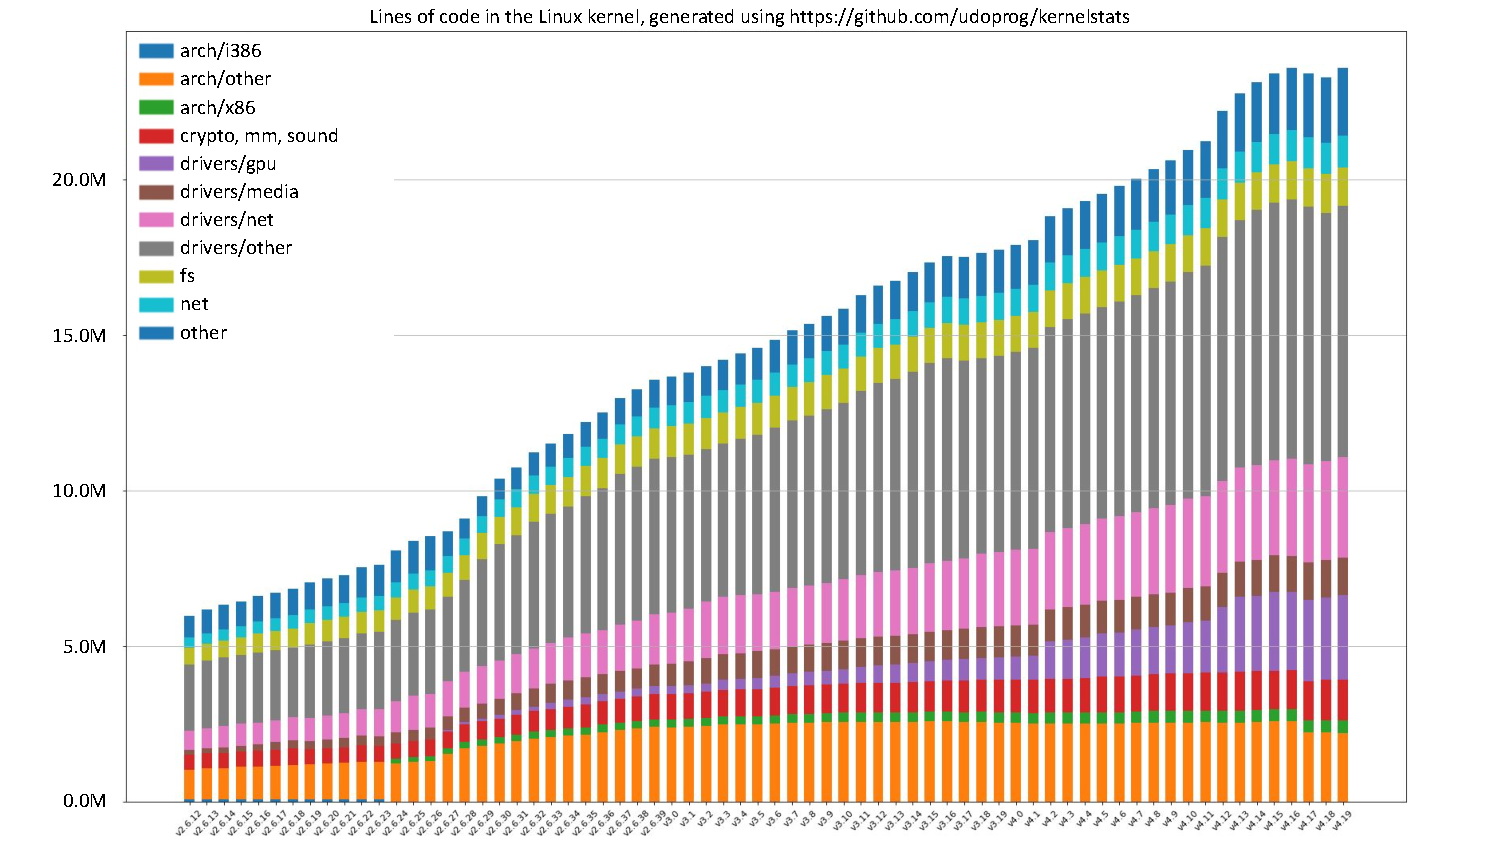
\includegraphics[width=\textwidth]{figures/linux-loc.pdf}
    \caption{Lines of code in each version of the Linux kernel \cite{kernel-stats}}
    \label{linux-growth}
\end{figure}

Linux is mostly written in the C language. While extremely fast and powerful, C does not offer support for useful object-oriented concepts. As a workaround, developers use structs within the Linux source code to mimic a semi object-oriented structure. Since a C struct can combine data items of different kinds, the struct can hold multiple data values, representing the attributes of an object, and multiple pointers to functions, representing the methods of an object \cite{c-struct}. Additional complexity like inheritance and polymorphism can also be achieved, offering great flexibility. However, this demands a good mastery of low-level technical concepts such as pointers, and is not particularly readable. 

The readability issues were compounded by the complexity of the transition to multicore. Had the developers had the opportunity to design Linux with multicore in mind from the outset, the design could have been simpler, because they would not have been constrained by the existing codebase. Redesigning an established operating system retrospectively is not a feasible option either; the cost of redeveloping Linux was estimated in 2011 at \$3 billion USD \cite{linux-kernel-cost}, and again in 2018 at \$14.7 billion USD \cite{cost-to-redev}. To further compound the readability issues, the Linux documentation is not yet complete, with the community still working to integrate separate documents into a coherent whole \cite{linux-docs}. In essence, while being a freely-accessible example of an established operating system, Linux is not easily understood.

\subsection{RTOS}
Real-time operating systems are a class of operating system that demand strict performance guarantees. Examples include safety-critical systems such as air traffic control systems, where data provided by sensors must be processed and responded to immediately. Processing must therefore be done within specified time constraints, or the system will fail \cite{silberschatz}. The real-time scheduling provided by Linux and similar operating systems makes no guarantees of meeting these time constraints, whereas a dedicated RTOS like FreeRTOS \cite{free-rtos} will. However, the need to maintain these guarantees heavily restricts scheduler development within the RTOS. Similar to Linux, InfOS makes no such real-time performance guarantees, giving us the flexibility to experiment with the scheduling interface without needing to maintain any strict performance assurances.

\subsection{Barrelfish}
The negative implications of retrospective multicore design are being recognised by researchers \cite{barrelfish-article}. Current operating systems were not designed to support computers with large numbers of cores, and researchers are beginning to explore radical new ideas, specifically focused on increasing scalability. One such project is a research operating system called Barrelfish \cite{barrelfish-website} that aims to explore a new paradigm for negotiating the multicore era. Barrelfish is written from scratch, removing the constraints that an operating system with an existing codebase bring. In particular, the researchers have proposed that having a shared-memory kernel with data structures protected by locks is a bottleneck. Rather than having small parts of the kernel stored in the caches of each processor and trying to maintain cache coherence, they instead experiment with a multikernel architecture. This is a distributed system with essentially one kernel per core, each having a replicated operating system state. The kernels explicitly communicate via message-passing and hardware keeps the replicated states consistent. The project also recognises the increasing diversity in computer hardware, and focuses on designing the operating system structure to be independent of particular hardware characteristics, increasing portability. 

\section{Motivation} \label{motivation}
InfOS \cite{infos} is a research operating system, written entirely from scratch in C++ following an object-oriented design. It is based on the x86 architecture, and was designed and developed by Tom Spink for the UG3 Operating Systems course \cite{ug3os}, although it is technically a general purpose operating system. InfOS was designed precisely because modern operating system kernels like the Linux kernel are extremely complex and difficult to understand. It is a valuable teaching tool that forms the foundations of the Operating Systems coursework and provides interfaces for core operating system operations. This allows students to rewrite different subsystems, like the memory allocator or the scheduler, and develop their understanding of operating system internals. 

InfOS currently only supports unicore processing, but being relatively lightweight in comparison to large-scale and long-lived operating systems, InfOS presents a rare opportunity to redesign an operating system specifically with multicore processing in mind. The object-oriented design of InfOS will extend naturally to support multicore processing in a well-structured manner, and adding this support will develop InfOS further as a teaching and research tool. Unlike the Barrelfish project, which aims to explore radical new multikernel structures for operating systems, InfOS aims to take the familiar and well-established monolithic kernel structure and provide the following key contributions.

\subsection{Key Contributions} \label{key-contributions}
\begin{description}
    \item [Teaching contributions.] A well-designed, object-oriented multicore operating system that can be easily understood by students. As discussed, multicore processing is a very pervasive field, and thoroughly understanding parallel architectures is vital for computer science students, especially those interested in systems development. InfOS follows a conventional operating system structure, meaning that students' understanding can be mapped to larger systems such as Linux.
    \item [Technical contributions.] A working operating system implementation that can be downloaded by anyone, booted on real hardware and used to execute user programs.
    \item [Research contributions.] A platform on which to build further research. The multicore implementation will extend the way InfOS provides interfaces for components of the operating system, allowing experimentation with different algorithms for load balancing and performance optimisation. Section \ref{transition-to-multicore} noted that a modular scheduler would be beneficial for experimenting with new algorithms, and we discuss our future research paper based on this idea in section \ref{future-work}.
\end{description}

\chapter{Implementation} \label{implementation}

\section{Existing System} \label{existing-system}
As described in section \ref{motivation}, InfOS has a clear advantage over other operating systems because it was specifically designed to be straightforward to understand. With this being said, InfOS is still a general purpose operating system, and the whole repository comprises around 20,000 lines of code. Before implementation could begin, the major conceptual challenge was to understand the existing system. There is a brief specification document \cite{os-cw-spec} written by the designer, which is aimed at students of the UG3 Operating Systems course. This document explains InfOS’s high-level structure and implementation, but it is by no means extensive technical documentation. Most of my understanding of InfOS therefore came from navigating the existing codebase and reading the Intel architecture manuals \cite{intel-full-manual}. This consumed a significant portion of development time throughout the entire project. Furthermore, since the C++ standard library implementation uses system calls, it must be ported to each individual operating system. Naturally, no such port exists for InfOS, meaning that the entire implementation had to be written in the C++ core language \cite{cpp-core}. Any standard C++ functionality needed during the implementation, including strings, lists, maps, input/output, random number generation, atomics support and time utilities, had to be written from scratch. This became particularly relevant during evaluation and benchmarking, when atomic operations were needed (see section \ref{mb-benchmark} for further details).
 
The Advanced Programmable Interrupt Controller (APIC) \cite{intel-sys-prog-guide} is the Intel standard for controlling interrupts, and InfOS follows this standard. The standard defines two main controllers, a local APIC (LAPIC) and an external input/output APIC (I/O APIC). The I/O APIC is responsible for receiving external I/O interrupts, such as keyboard strokes, and relaying them to the LAPIC. Each LAPIC has a LAPICTimer, and the LAPIC is responsible for receiving internal I/O interrupts such as LAPICTimer interrupts, alongside the I/O APIC generated interrupts. The APIC standard supports multiprocessor systems by representing each processor as a core and a LAPIC, with each LAPIC handling core-specific interrupts. With this representation, the system has one I/O APIC, and as many LAPICs and LAPICTimers as there are cores. Figure \ref{cores-lapics} shows an example in the case of a quad-core system. The cores may communicate by sending interprocessor interrupts (IPIs) from their LAPIC to another processor’s LAPIC \cite{intel-sys-prog-guide}. 

\begin{figure}[h]
    \centering
    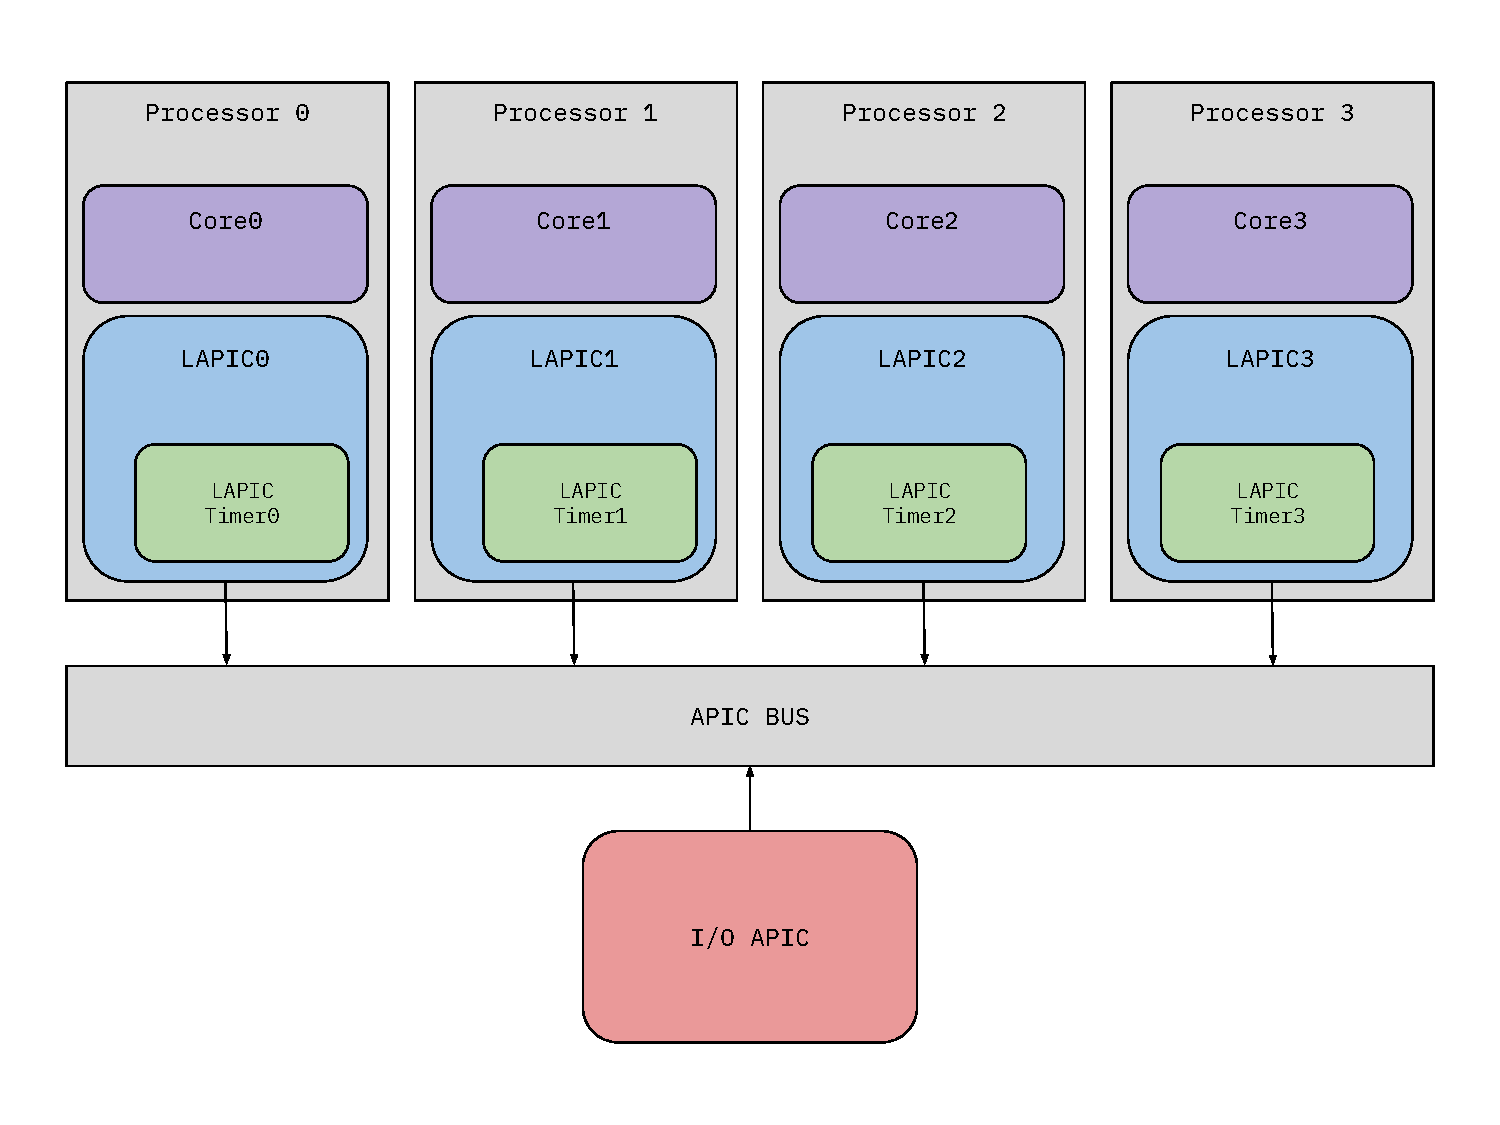
\includegraphics[scale=0.6]{figures/cores-lapics.pdf}
    \caption{Block diagram showing the APICs in a quad-core system}
    \label{cores-lapics}
\end{figure}


InfOS has an object-oriented design, with each of the major components of the operating system represented as a subclassed device object. For example, the scheduler, I/O APIC and LAPIC are all represented as devices. When InfOS boots, the platform is probed, and any detected devices are created and registered with a central device manager object. Every device is assigned a unique name by the device manager, who is then responsible for providing an interface that allows any class of device to be accessed by other parts of the system. The most natural design extension was to represent the cores as objects, with each core having a separate LAPIC and LAPICTimer object. With this design in mind, I broke the implementation down into four main milestones:

\begin{description}
\item [Detecting cores.] QEMU \cite{qemu} is a virtualisation environment that can be used to boot real operating systems in a virtual machine. It can be used throughout development to emulate running InfOS with varying numbers of cores. The first milestone, then, is to supply InfOS with multiple cores and detect those cores during boot.

\item [Initialising cores.] Recall from section \ref{architectural-challenges} that the x86 ISA defines a MP initialisation protocol, which defines two classes of processors, the bootstrap processor (BSP) and application processors (APs). The BSP runs the main operating system boot code, and is responsible for the detection of other cores. The APs are initially in a waiting state, so the BSP is also responsible for sending them a memory address to start execution at. For the purpose of this milestone, the code can be general code, such as “Hello world from core x!”.

\item[Calibrating timers.] InfOS supports preemptive scheduling by having the LAPICTimer generate interrupts every 4 milliseconds, which then trigger scheduling events. To extend this, each core’s LAPICTimer must be calibrated and initialised to send periodic interrupts too. The calibration code determines the frequency of the timer by measuring it against the programmable interrupt timer (PIT), meaning that the calibration code must be executed on the core itself in order to determine the correct frequency. Therefore, the earliest point at which the timer calibration can be done is once each core is awake and running general code, so this is the third milestone.  

\item[Scheduling threads.] On every timer interrupt, a scheduling event occurs, so the next logical step is to configure the scheduler to recognise multiple cores and dispatch tasks between them. Once this is implemented, all threads running in the operating system will need to be shared between the cores. This introduces a lot of design decisions, such as how to distribute the threads between the cores and whether a centralised scheduling manager should be used to coordinate.
\end{description}

\section{Detecting Cores} \label{detecting-cores}
As already mentioned, QEMU provides a simple way to modify the number of cores available to InfOS via the \verb|-smp| argument. For instance, InfOS can run on a dual-core processor by adding the command line argument \verb|-smp 2| to the runscript. Once provided with multiple cores, however, InfOS still has to detect them. The Advanced Configuration and Power Interface (ACPI, not to be confused with the previously mentioned Advanced Programmable Interrupt Controller, APIC) provides an open standard that operating systems can use to discover and configure hardware components. To begin using ACPI, the operating system must locate the Root System Description Pointer (RSDP), which contains a pointer to the Root System Description Table (RSDT), which contains pointers to yet more tables describing the hardware available on the system. InfOS already had an implementation to locate the RSDP, enable ACPI and parse the tables, so I extended this existing code to collect information about the available cores. 

One of the tables pointed to by the RSDT is the Multiple APIC Description Table (MADT), which describes all of the interrupt controllers in the system. Each entry in the MADT has an entry type, and entry type 0 is used to represent LAPICs, as shown in figure \ref{madtentry0}. 

\begin{figure}[h]
    \centering
    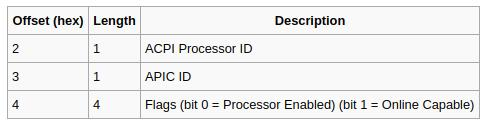
\includegraphics[scale=0.7]{madtentry0.jpg}
    \caption{MADT Entry Type 0 \cite{osdev-madt}}
    \label{madtentry0}
\end{figure}

Since each core has a LAPIC, each core's LAPIC will be represented by one individual MADT entry of type 0. Each entry contains the processor's ID, the LAPIC's ID and a set of flags. The flags are represented as 32 bits (see figure \ref{entry0flags}) and contain extremely important information: whether or not the processor can be enabled. If bit zero is set, the processor is enabled. If bit zero is clear, but bit one is set, then the system supports enabling the processor during runtime. If neither bit is set, then there is some error with the processor, meaning that it cannot be enabled and the operating system should not try.

\begin{figure}[h]
    \centering
    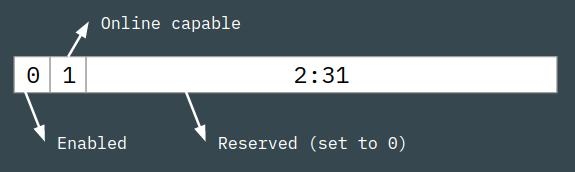
\includegraphics[scale=0.6]{figures/entry0flags.jpg}
    \caption{Entry type 0 flags structure}
    \label{entry0flags}
\end{figure}

It is useful to know which core is the BSP (for timing purposes, discussed further in section \ref{calibrating-timers}), so this information needs to be recorded at some point during core detection or core initialisation. The simplest way is to record the ID of the BSP, which can be done by reading the ID register of the BSP's LAPIC. Every core's LAPIC registers are memory-mapped to the same base address, and this base address is specified in the MADT. This mapping means that each core is only able to directly access its own LAPIC registers, so reading the BSP's LAPIC ID register must be done by code executing on the BSP. At this stage of boot, only the BSP is executing code while the APs sit idle, so the core running the code parsing the ACPI tables is guaranteed to be the BSP. For this reason, it makes sense to collect the BSP ID at this point by reading the LAPIC ID register, and store it for later.

As already discussed, the object-oriented design of InfOS extends well to supporting multiple cores. I decided to represent each core as a new subclass of device, creating and registering a new core object with the device manager whenever an entry type 0 was encountered in the MADT table. Within the core object, I stored the LAPIC ID, needed later for sending IPIs between cores, and the core state. The core state is represented by an enum with four values, \verb|BOOTSTRAP|, \verb|ONLINE|, \verb|OFFLINE|, and \verb|ERROR|, and is used during the core initialisation process to decide whether or not to send the wake sequence of IPIs to the core. If bit zero and bit one are both clear, the core state is set to \verb|ERROR| so that the core is not enabled later. Otherwise, the core's state is set to \verb|OFFLINE|, with this being changed to \verb|ONLINE| once the initialisation sequence is complete. The only exception is the case when the core's ID matches the BSP's ID, in which case the state is set to \verb|BOOTSTRAP|. Note that state \verb|BOOTSTRAP| implies the state \verb|ONLINE|, since if we have reached this stage in the boot process, the BSP is already executing code. Figure \ref{state-flowchart} shows the parsing process as a flowchart.

\begin{figure}[h]
    \centering
    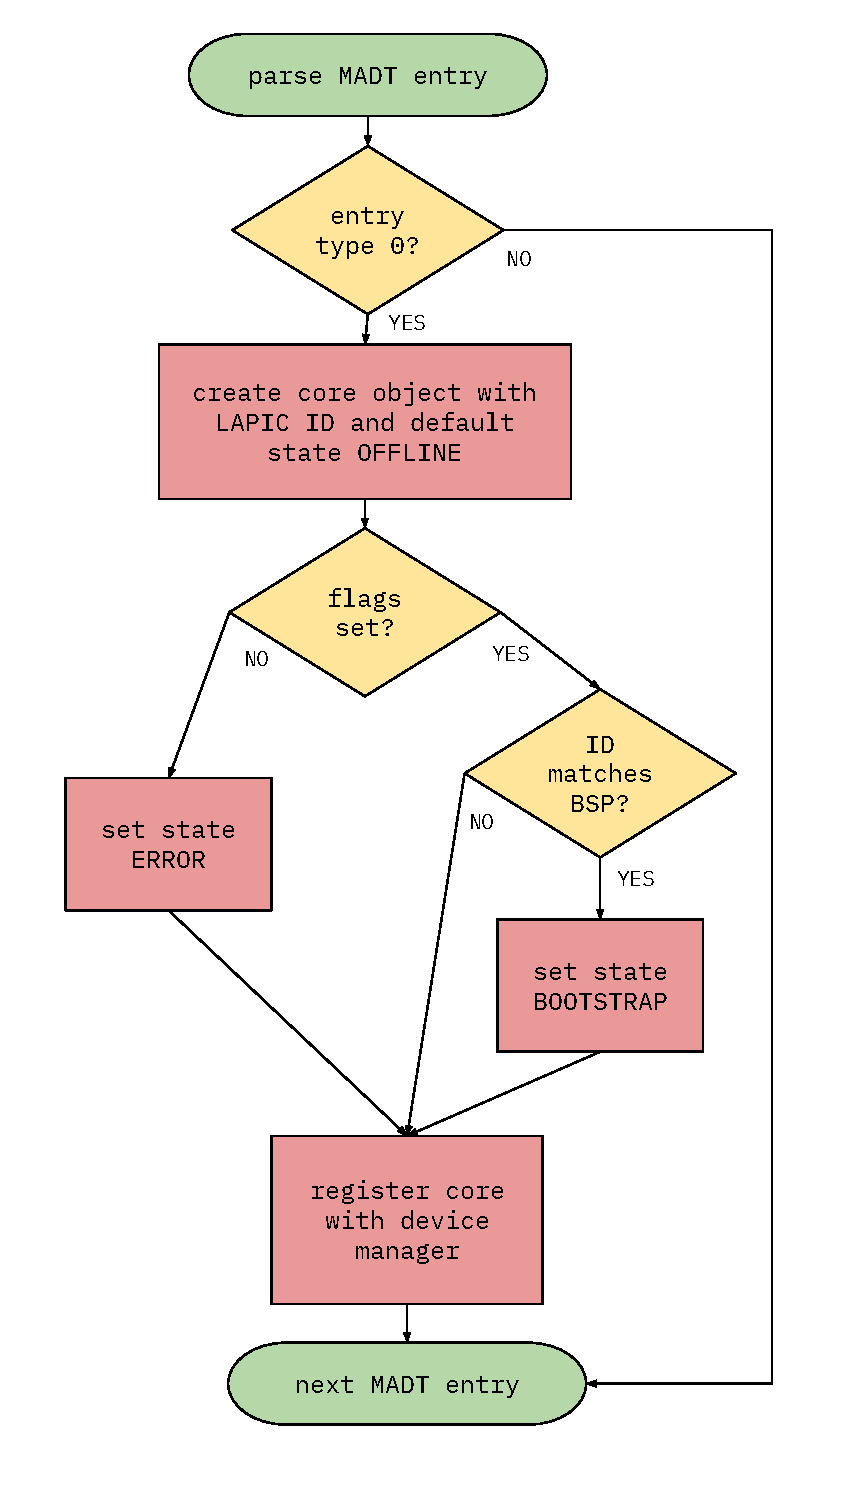
\includegraphics[scale=0.6]{figures/state-flowchart.pdf}
    \caption{Flowchart depicting the process of parsing MADT entries and creating core objects}
    \label{state-flowchart}
\end{figure}

 The core objects should be accessible from anywhere within InfOS to allow the operating system to make calls on them, so I added a \verb|cores| method to the device manager that iterates through all devices in the system, appends any of type \verb|Core| to a \verb|List<Core*>| returns the list. I also added a static mapping \verb|Map<uint8t, Core*> cores| in the \verb|Core| class that maps each core ID to the associated object, and a static function \verb|get_current_core| that reads the ID register of the currently executing core's LAPIC and returns the object instance mapped to by that core ID.

\section{Initialising Cores} \label{initialising-cores}
Once the APs have been detected, they need to be triggered to begin executing. The BSP can generate interprocessor interrupts (IPIs) by writing specific values to one of its LAPIC registers, the interrupt command register (ICR). As already mentioned, each core is able to directly access its own LAPIC registers by writing to the LAPIC base address plus some offset. The ICR comprises two 32-bit registers, one at offset \verb|0x300| and the other at offset \verb|0x310|. The Intel MP protocol defines a sequence of IPIs, called an INIT-SIPI-SIPI sequence, that wakes an AP from the waiting state. To send an Initialisation (INIT) IPI, the BSP first writes the target LAPIC ID into bits 24-27 of offset \verb|0x310|, then writes the value \verb|0x00004500| to offset \verb|0x300|, which generates the interrupt. To send a Startup IPI (SIPI), the target LAPIC ID is written as before, and then the value \verb|0x00004600| is or-ed with the page number at which the AP should begin executing, before being written to offset \verb|0x300|. The initialisation sequence then proceeds as follows: the BSP sends an INIT IPI to the AP, waits 10 milliseconds, sends a SIPI and then waits a further 1 millisecond. The BSP then polls for a ready flag from the AP indicating that it is online. If the ready flag is not set, the BSP repeats the SIPI and waits a further 1 second. If the ready flag is still not set after the second SIPI, the core state is set to \verb|ERROR| and the BSP stops trying to wake that core. Figure \ref{init-sipi-sipi} depicts the INIT-SIPI-SIPI sequence as a flowchart.

\begin{figure}[h!]
    \centering
    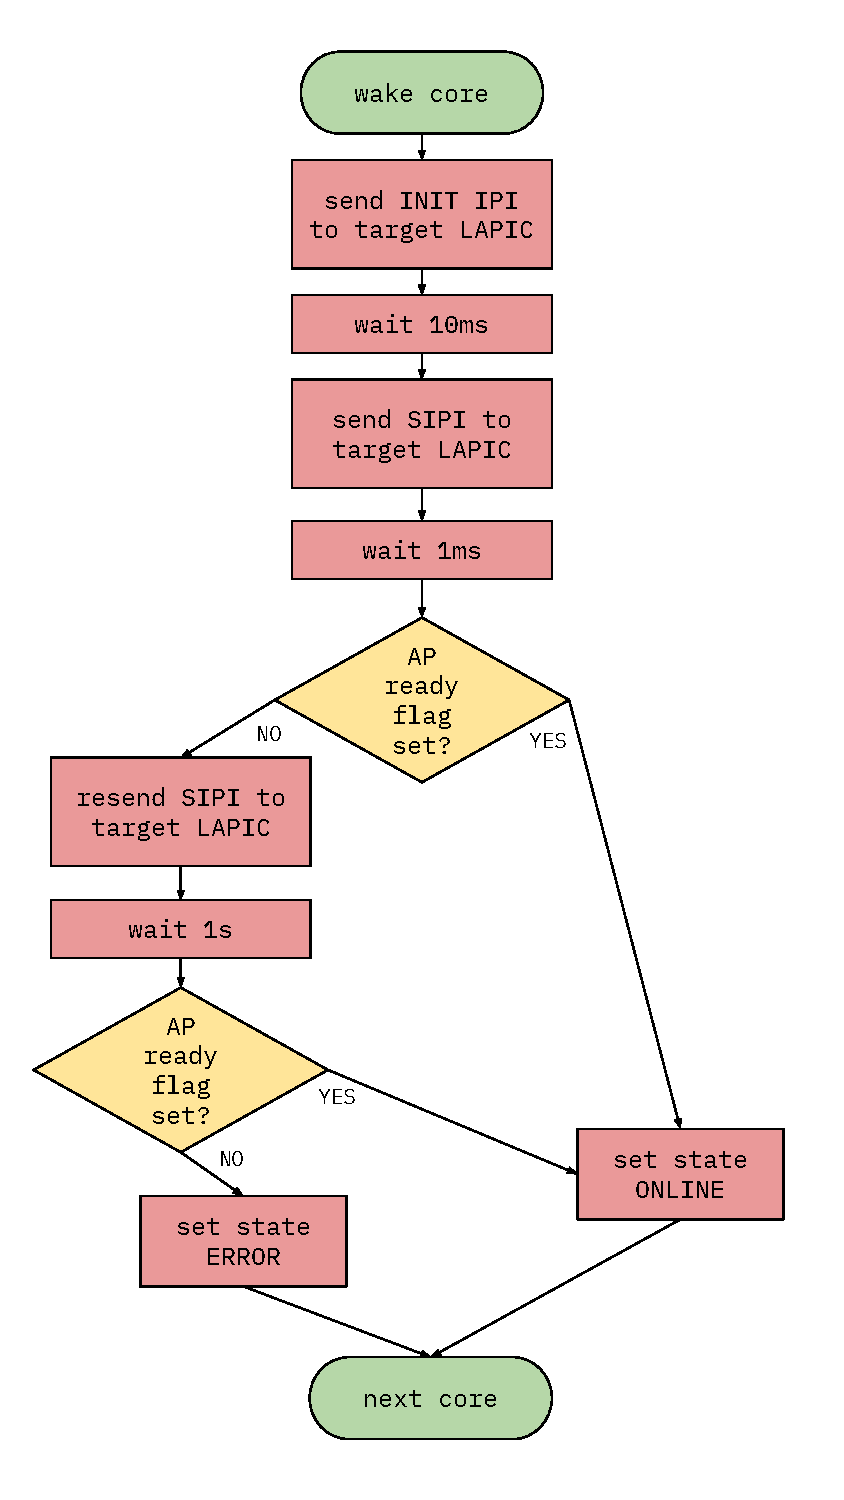
\includegraphics[scale=0.6]{figures/init-sipi-sipi.pdf}
    \caption{Flowchart depicting the INIT-SIPI-SIPI sequence for waking each core}
    \label{init-sipi-sipi}
\end{figure}

The page address sent with the SIPI locates initialisation assembly code, commonly referred to as trampoline code. The BSP allocates page zero as the trampoline page and copies the assembly code onto that page, before including the address of that page with the SIPI. For compatibility reasons, all x86 processors begin execution in 16-bit real mode, a simplistic mode used by early operating systems with only 1MB of addressable memory, no memory protection and no virtual memory. The main operating mode of Intel processors today is 64-bit protected mode, so the trampoline code must enable this on the AP. In protected mode, memory access is controlled through the Global Descriptor Table (GDT), which stores information about various memory areas, their base address, size and access privileges. Therefore, before entering protected mode, the AP must first prepare a temporary GDT to access. Once the GDT is ready, 32-bit protected mode is enabled by setting the \verb|PE| control flag in the \verb|CR0| register. 

From 32-bit mode, the AP then jumps to 64-bit protected mode. However, it has not yet finished initialising. In a similar fashion to memory access, interrupt handling is controlled through the Interrupt Descriptor Table (IDT), so the AP must also load this table using the \verb|lidt| instruction. The LAPIC is an interrupt controller, and it controls interrupt redirection by accepting interrupt requests and feeding them to the processor. Without an interrupt controller, the processor would have to poll all of the devices in the system to see if they require attention. The LAPIC replaces the older 8259 Programmable Interrupt Controller (PIC), which did not support sophisticated interrupt redirection or IPIs \cite{osdev-apic}. However, the PIC is enabled for legacy reasons, so the trampoline code must also disable the PIC to prevent interference with the LAPIC. 

Additionally, InfOS uses paging, so this must be enabled on the AP. However, before paging is enabled, the page directory address needs to be loaded into the AP's \verb|CR3| register so that the AP can locate the page table. The trampoline code reserves some storage space for this value in the data segment, and then the BSP inserts this value when copying the trampoline code to page zero. The AP then loads this value from the data segment into its \verb|CR3| register, and paging is enabled by setting the \verb|PG| flag in the \verb|CR0| register. Furthermore, each AP needs its own stack, so the BSP allocates the AP one page of memory and again inserts a pointer to this page in the data segment. The AP can then load this value into its \verb|RSP| register, at which point, the AP is finished using the trampoline code. There is one final reserved storage location for the previously mentioned ready flag, which the AP sets and the BSP polls for. Finally, the AP jumps to a function \verb|x86_core_start|, which prints \verb|"Hello world from core x!"| to the terminal and then pauses indefinitely. A six core system (with one BSP and five APs) would give the console output shown in figure \ref{hello-world}.

\begin{figure}[h]
    \centering
    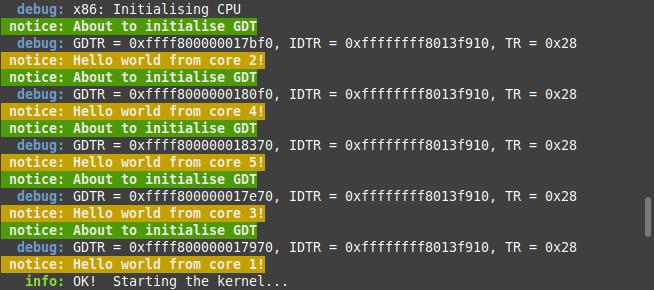
\includegraphics[scale=0.6]{figures/hello-world.jpg}
    \caption{Console output when initialising a six core system}
    \label{hello-world}
\end{figure}

The sequence described above needs to be done for each core individually, and this can either be done in serial or in parallel. Serial initialisation has one trampoline page that each AP uses in turn, with the BSP waiting for one AP to complete initialisation before sending the INIT-SIPI-SIPI sequence to the next AP. This introduces a bottleneck that could be reduced by giving each AP a separate trampoline page and broadcasting the INIT-SIPI-SIPI sequence across the bus to start all present cores. However, this will wake any present core, irrespective of the value of the core's ready flags found in the MADT, which could potentially wake a core that had been deliberately disabled due to an error. For this reason, other operating systems generally avoid broadcasting during AP initialisation, and I took the same approach. Instead, the BSP retrieves the list of available cores and only sends IPIs to \verb|OFFLINE| cores. The BSP has to then wait for each core to set the ready flag before knowing whether to resend the SIPI, or move on and update the core's state. The initialisation code is relatively small because InfOS is so lightweight, meaning that this serial initialisation process has a negligible impact on overall system performance. 

All of the code described above is contained within two small methods, \verb|cpu_init| and \verb|start_core|, which are executed during the boot process by the BSP. The function \verb|cpu_init| requests a reference to the BSP's LAPIC object and the Programmable Interval Timer (PIT) from the device manager. It then retrieves the list of cores from the device manager and iterates through it, calling \verb|start_core| whenever a core should be initialised. The LAPIC class has methods \verb|send_remote_init| and \verb|send_remote_sipi| that write the appropriate values to the LAPIC registers to generate the IPIs, and the BSP calls these functions on its own LAPIC object within the \verb|start_core| function. The PIT has a function \verb|spin| which initialises one-shot mode (see section \ref{calibrating-timers}) and issues \verb|nop| instructions until the timer stops. This function is used when the BSP needs to wait a certain number of milliseconds as described above.

\section{Calibrating Timers} \label{calibrating-timers}
Recall that each AP has a LAPIC and a LAPICTimer, which need to be initialised and registered with the device manager. This initialisation involves reading and writing the LAPIC registers, so it had to be delayed until the APs were executing code so that it could be done locally. The first step is to create a LAPIC object for the AP and register it with the device manager. Since every core in the system would be repeating this, it made sense to write a method \verb|lapic_init| within the core object. This method reads the LAPIC base address collected when parsing the MADT tables, creates a LAPIC object and registers it with the device manager. All device objects must implement a method \verb|init|, which the device manager calls when registering a new device. To enable the LAPIC to receive interrupts, it is necessary to configure the Spurious Interrupt Vector Register with the IRQ number to map spurious interrupts to, so the LAPIC \verb|init| function does this. Finally, since the LAPIC object is needed whenever the core wants to read its LAPIC registers or send IPIs, the core object also stores a reference to its LAPIC object. 

Once the LAPIC object has been created, it can be used to create and calibrate the LAPICTimer object. Since InfOS is preemptive, each AP's LAPICTimer needs to be initialised to tick periodically, generating timer interrupts to tell the AP when to schedule. The LAPICTimer has two modes. Periodic mode has an initial count set by software, and the LAPICTimer decrements this count until it reaches zero, generates an interrupt and then resets the current count to the initial count and begins decrementing again. One-shot mode decrements the initial count in the same way as periodic mode and generates an interrupt when it reaches zero, but it does not reset the current count. If another one-shot interrupt is required, the software must set the initial count again. The advantage of each core having a LAPICTimer is that cores don't have to share the Programmable Interval Timer (PIT), which lies on a separate circuit. The disadvantage is that while the PIT uses a standard frequency, the LAPICTimer's frequency varies from machine to machine, so it must be determined before the LAPICTimer can be used \cite{osdev-apic-timer}. To do this, the LAPICTimer can be reset to a well-known state and calibrated using the PIT as a reference timer. 

I defined a second function within the core object, \verb|timer_init|, to do this. This function creates the LAPICTimer object, passing a reference to the associated LAPIC object. The function then registers the LAPICTimer with the device manager, which calls the LAPICTimer's \verb|init| function. This init function calibrates the timer by initialising both the LAPICTimer and PIT for one-shot operations, then counting the number of LAPICTimer ticks that happened during that period and calculating the frequency. InfOS's frequency is 250Hz, so the LAPICTimer should be set to interrupt the AP every 4 milliseconds. The LAPICTimer object defines \verb|init_periodic| and \verb|start| functions, which make calls on the associated LAPIC object to write values to the registers. Once the timer is calibrated, the \verb|timer_init| function sets the timer to be periodic, with a period of 4ms, and starts the timer using these functions. As previously mentioned, this code needs to be executed locally on the AP. The previous milestone had the AP jump to a function \verb|x86_core_start| that printed to the terminal and entered an infinite loop of \verb|nop|, so I modified this function to call \verb|lapic_init| and then \verb|timer_init| on the core object, which the BSP passed the AP a reference to through the trampoline code.

In section \ref{detecting-cores}, I mentioned that it was important to record which core is the BSP. This is because in the unicore case, the kernel updated the system runtime with 4ms on every timer interrupt. However, with multiple cores, this would be done for every 4ms for every core, making the system runtime wrong by a factor of the number of cores. Within the timer interrupt handler, I retrieved the current core object by calling the static method \verb|get_current_core| in the \verb|Core| class, and added a conditional to only update the system runtime if the state of the current core is bootstrap.

Again, the above timer calibration steps needed to be done for each core. This time, it seemed natural to have all cores initialising themselves in parallel since the initialisation was done locally on each core. The only consideration was regarding synchronising access to the PIT and the device manager. This was necessary because each core registers devices with the device manager, which involves modifying a global list of devices, and because each core uses the PIT to calibrate its LAPICTimer. Furthermore, recall that the BSP uses the PIT for spin delays while initialising the APs, which increases contention on the PIT. For example, a previously started AP could be using the PIT to calibrate while the BSP is spin-waiting for the next AP to come online. I addressed this by protecting the PIT and the global devices list with two spinlocks. When the device manager wishes to add a device to the list, the device manager lock is acquired, the device is added, and then the lock is released. When the PIT function \verb|start| is called, the PIT lock is acquired, and when the PIT function \verb|stop| or \verb|reset| is called, the lock is released. The PIT functions \verb|spin| and \verb|init_oneshot|, used by the BSPs and the APs respectively, then utilise these \verb|start|, \verb|stop| and \verb|reset| functions.

% One optimisation here would be to use mutexes rather than spinlocks. The difference is that when a spinlock cannot be acquired, it enters a busy waiting period, which is essentially where the lock is tested in a loop until it can be acquired. When a mutex cannot be acquired, the thread trying to acquire the lock will yield the processor, and the lock will not be tested again until the thread gets its next timeslice. This means that while a thread is waiting for the lock, CPU cycles are not being wasted on busy waiting, but instead are being used to make progress on other threads. However, yielding requires the thread's context to be saved and a schedule event to occur. At this point, the scheduler has not yet been adapted to handle the multiple cores, so a mutex is not a viable option. If the scheduler was initialised before the timers, this would have been possible, but this would have required significant rearchitecture of the system's boot process, possibly sacrificing readability. The use of spinlocks here is acceptable, since the spinlock will only be held for a very short period of time, limiting the impact on the system's performance.

\section{Scheduling Threads} \label{scheduling-threads}
Once the cores were taking timer interrupts at the correct frequency, the final piece of the puzzle was to configure a scheduling event to happen on these interrupts. Section \ref{scheduling-challenges} mentioned that there are two approaches to scheduling: either a per-core runqueue, or a system-wide runqueue. A system-wide runqueue would have to be protected with locking to prevent race conditions. However, locking adds significant overhead, since it prevents any of the other cores from progressing while one core holds the lock. This overhead would be included in every schedule event, which happens on every AP's timer tick, or every 4 milliseconds. The more cores in the system, the more critical this bottleneck becomes. With scalability in mind, the only realistic option is therefore to have multiple, per-core runqueues.

Before discussing the implementation, I will explain how InfOS previously handled scheduling in the unicore case. Processes were represented as a class, and were each allocated an area of virtual memory. The process then had a variable \verb|main_thread| that was initialised when the process was created. The process also had a list of thread objects, allowing processes to be multithreaded if required, and a method \verb|create_thread| that allowed adding new threads. Threads therefore existed within the context of a process, and shared the address space with other threads belonging to the same process. Threads were also represented as an object, with a reference back to their process parent and an associated stack and context. InfOS focuses on threads when scheduling, and the thread class is wrapped with a scheduling entity class that holds properties such as the current runtime and the scheduling state. The scheduling state could be either \verb|STOPPED|, \verb|SLEEPING|, \verb|RUNNABLE| or \verb|RUNNING|.

There was one global scheduler object with a reference to a scheduling algorithm, which was an interface that managed the system-wide runqueue. The interface provided methods such as \texttt{pick\_next\_task}, \texttt{add\_to\_runqueue} and \texttt{remove\_from\_runqueue}. Different scheduling policies, such as first-in-first-out, round-robin, or Linux's CFS could then implement the interface, and the user could select between them at boot-time using command line arguments. The scheduling algorithm worked with scheduling entity objects, meaning that although InfOS currently schedules threads only, the concepts are kept separate and InfOS could easily be switched to schedule processes (like Windows), or processes and threads (like Linux). This can be seen in figure \ref{schedulers}.

\begin{figure}[h]
    \centering
    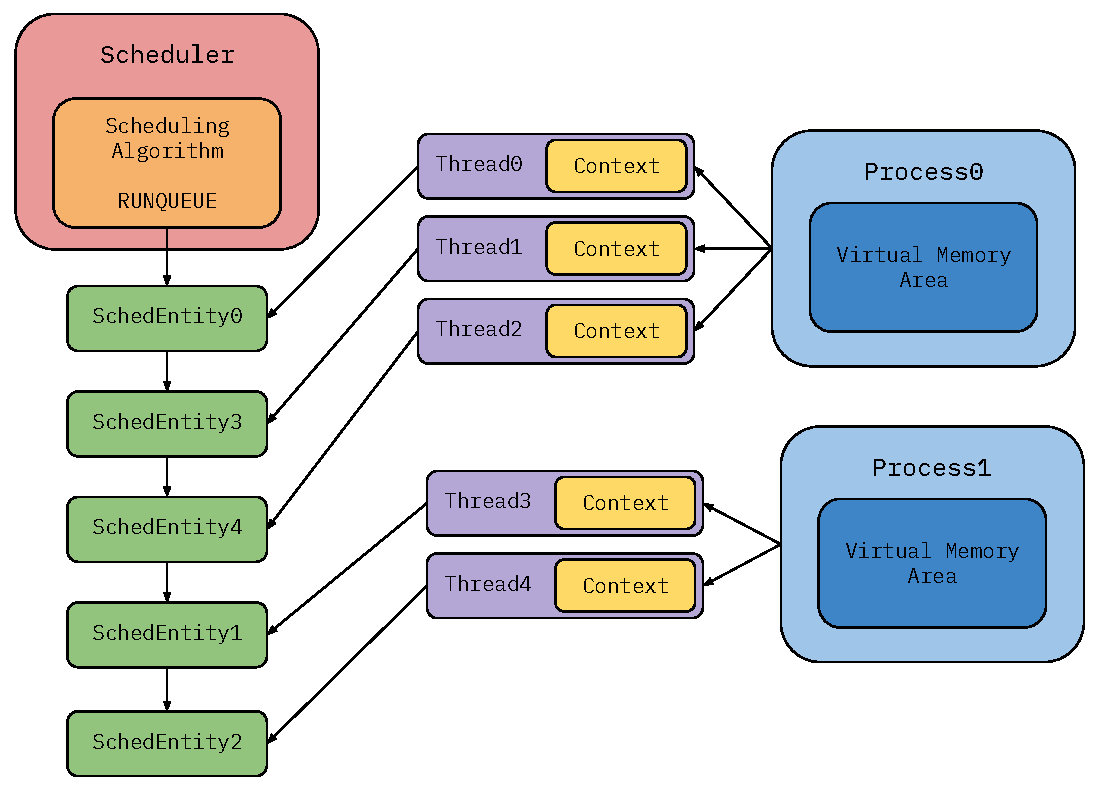
\includegraphics[scale=0.7]{figures/schedulers.pdf}
    \caption{Block diagram depicting the scheduler components within unicore InfOS}
    \label{schedulers}
\end{figure}

The scheduler initialisation happened during boot, and involved creating the scheduler object, an idle process and an idle thread. The idle thread is essentially a function that pauses indefinitely by issuing the \verb|pause| instruction, which was chosen over the \verb|nop| instruction because in the case of hyperthreading,  \verb|pause| lets the sibling core continue executing, whereas \verb|nop| wastes cycles. After the idle thread was created, it was activated, which set a global variable \verb|current_thread| to be that thread. This means that when the scheduler started running, the context that began being saved and restored was that of the idle thread. Once the kernel had finished the boot process, a \verb|run| function was called on the global scheduler, which essentially activated the first eligible thread, which would likely be the idle task. From that point onwards, on every timer tick, a function \verb|schedule| was called on the scheduler, and this function requested the next entity from the scheduling algorithm via \verb|pick_next_entity|. If the runqueue was empty, the algorithm returned \verb|NULL|, and the scheduler continued to schedule the idle thread. Otherwise, if a new thread had been created and added to the runqueue, the algorithm would return this and the scheduler would need to perform a context switch. This was done using the global \verb|current_thread| variable mentioned earlier, by saving the context of the previous thread and setting the variable to be the new thread. Naturally, this global variable would need to be refactored to support multiple cores, otherwise they would keep overwriting the current thread of the other cores.

In order to support the per-core runqueues but maintain the object-oriented structure, I decided to have one scheduler object per core. I refactored the core class to hold a reference to this scheduler object, and refactored the scheduler object to hold the \verb|current_thread| variable, rather than having one global \verb|current_thread|. Rather than initialising the scheduler once at the beginning of the boot process, the scheduler of each core needed to be created and initialised with an idle task as above. However, the BSP needed a functioning scheduler before initialising the APs in order to schedule the kernel thread running the boot code. I refactored the original scheduler initialisation code to initialise the BSP's scheduler rather than a global scheduler, and then delayed the AP scheduler initialisation until later in the boot process when the APs were online.

\begin{figure}[t!]
    \centering
    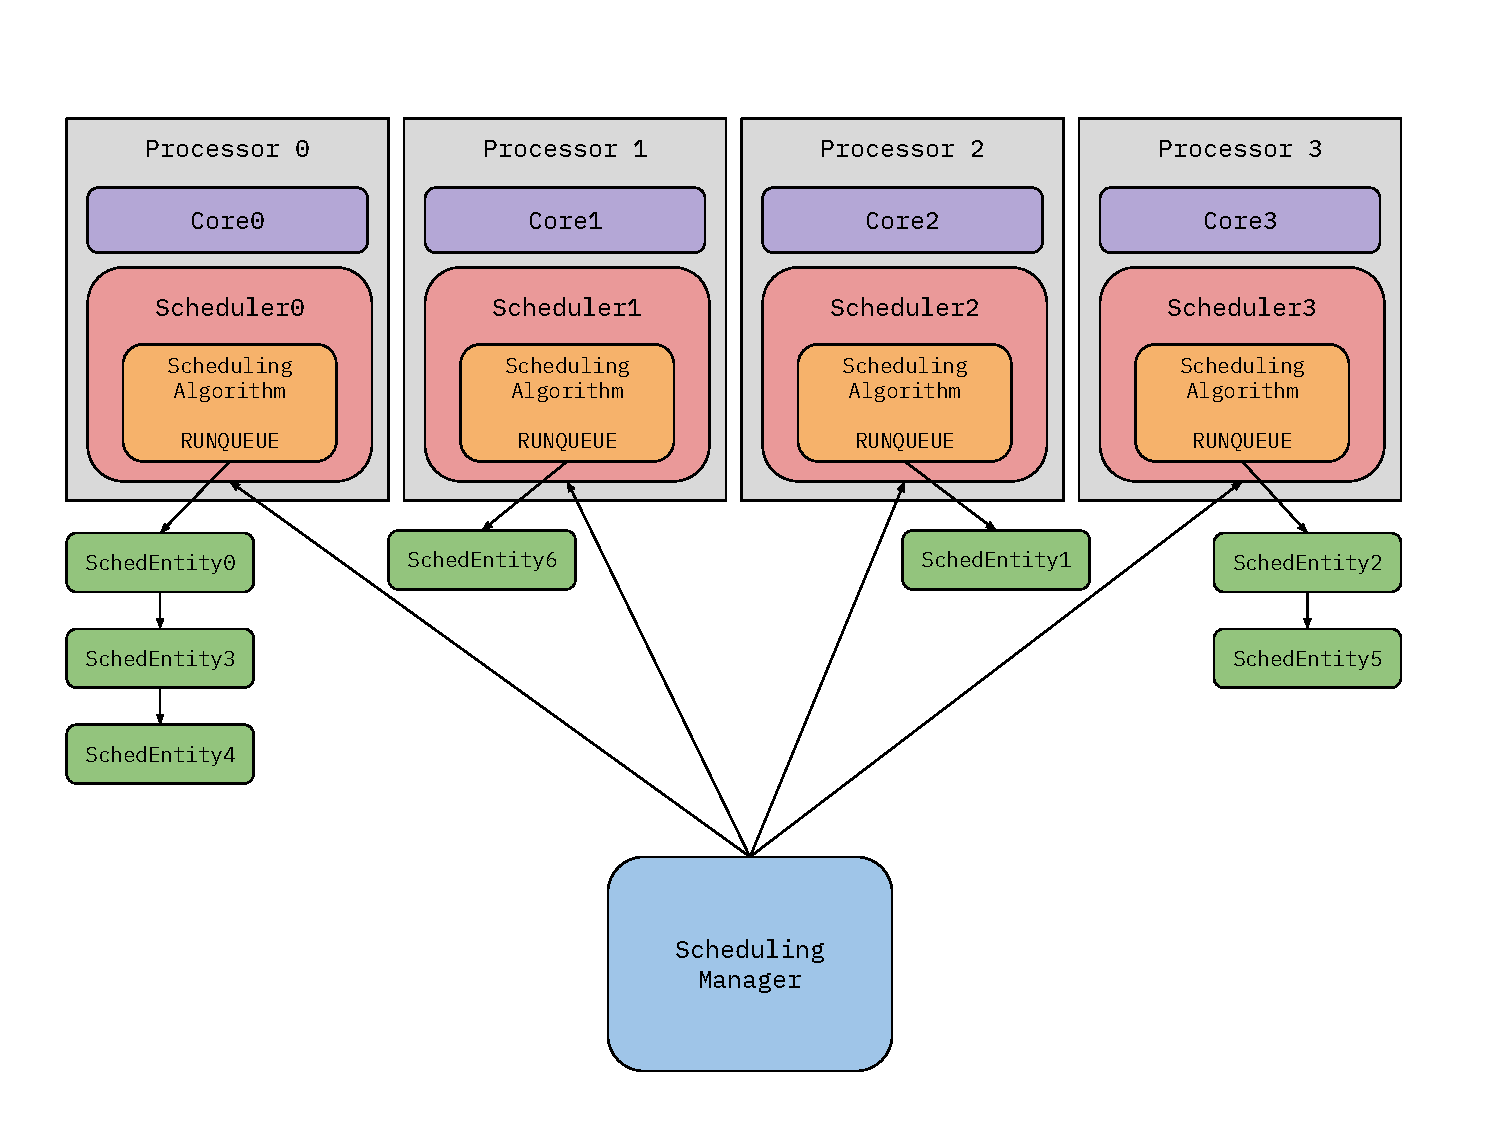
\includegraphics[width=\textwidth]{figures/multicore-schedulers.pdf}
    \caption{Figure depicting the scheduler components within a quad-core system}
    \label{multicore-schedulers}
\end{figure}

I do this scheduler initialisation as soon as the APs are online and executing code, so at the same time as the timer initialisation in section \ref{calibrating-timers}. They call the \verb|init| function on their scheduler object, which creates a new idle process and thread for that core and activates it. Then, they call \verb|run| to activate their schedulers once all initialisation has been completed, and this represents the point at which the core is fully initialised and begins scheduling threads. On every timer tick, rather than calling \verb|schedule| on the global scheduler, the function \verb|get_current_core| returns the current core object, which is then used to get a reference to the current scheduler. The function \verb|schedule| is then called to select a new task for that specific core, and perform the context switch as before.

When a thread was created previously, it would be added to the runqueue of the global scheduler object. With the removal of this object, there needed to be some way for new threads, or threads waking up from sleep, to be scheduled onto some core. I could have just added the thread to the runqueue of whatever core created it, but this would be a really obvious way to create a workload imbalance. When InfOS boots, the shell launches and waits for the user to run a program. The shell thread would likely be running on the BSP core, and then any program that the user launched would also be added to the BSP's runqueue, while all other cores sit idle. The system therefore needed some sort of global scheduling manager to distribute new tasks between cores, and then once a thread is assigned to a core, the core's individual scheduling algorithm could be responsible for distributing that core's cycles between the threads on that core's runqueue.

I created a global scheduling manager class which maintains a list of all schedulers in the system. Figure \ref{multicore-schedulers} shows the scheduler components within a quad-core system. On initialisation, each scheduler now registers itself with the scheduling manager, and this global scheduler list is protected with a mutex lock. When a new thread is created or awoken, the thread is passed to the scheduling manager, who then selects a scheduler and dispatches the task to that scheduler. I chose to mimic the abstraction provided by the scheduling algorithm class, and created a core algorithm command line parameter. The user can then specify how tasks should be distributed between cores, whether that be randomly or by some other metric (discussed further in section \ref{future-work}). This modular functionality allows easy customisation and fine-tuning of the scheduler's policy to tailor the system's performance to its workload.

% Todo: Something about IDT and GDT \\
% Also, all use the same type of  sched algorithm (different instances), created at boot. Could possibly be refactored to have different cores use different policies if there was some desire for that

\chapter{Evaluation}
As discussed in section \ref{scalability-challenges}, in order to fully exploit the processing power of multiple cores, software needs to be highly adapted to a parallel execution environment. An embarrassingly parallel problem is one where very little effort is needed to divide the original task into a set of almost independent parallel tasks, and such problems are both pervasive in computing and well-suited to exploiting parallel architectures. 

\begin{figure}[h]
    \centering
    
\includegraphics[scale=0.17]{mandelbrot-bw.jpg}
    \caption{Black and white rendering of the Mandelbrot set \cite{mandelbrot-bw}}
    \label{mandelbrot-bw}
\end{figure}

\section{The Mandelbrot Set}
The Mandelbrot set is the set of complex numbers $c$ for which the recurrence relation $f_{c}(z) = z^2 +c$ with $z_{0}=0$ does not diverge. Thus, a complex number $c$ is a member of the Mandelbrot set if, when applying $f_{c}$ repeatedly, the absolute value of $z_{n}$ remains bounded for all $n>0$. The set can be represented visually in a two-dimensional plane by taking each $(x,y)$ point in the plot as the real and imaginary parts of a complex number $c$, such that $c=x+iy$, and iteratively computing values for the recurrence relation $f_{c}$. An arbitrary escape value is chosen, and each iteration checks whether the result has exceeded this critical value. If the escape value has been exceeded, the computation has diverged and that pixel is not a member of the Mandelbrot set, so computation for that particular pixel can terminate. Otherwise, computation continues until a number of maximum iterations, at which point it is inferred that the pixel will probably not diverge and is a member of the Mandelbrot set. A simple black and white rendering like figure \ref{mandelbrot-bw} can then colour a pixel black if it does not diverge, or white if it does diverge. A coloured rendering can provide additional detail by recording how many iterations it takes each pixel to diverge and colouring each pixel correspondingly. This gives a representation of how fast each pixel diverges, as shown in figure \ref{mandelbrot-vis}.

\begin{figure}[h]
    \centering
    
\includegraphics[scale=0.7]{mandelbrot.jpg}
    \caption{Coloured rendering of the Mandelbrot set \cite{mandelbrot-set}}
    \label{mandelbrot-vis}
\end{figure}

The algorithm described above is often known as the escape time algorithm \cite{mandelbrot-plotting-algorithms}. It is a perfect example of an embarrassingly parallel problem, because the computation of each pixel is independent from every other pixel in the plane. Separate threads within InfOS can therefore handle the computation of each pixel without the need for any communication, making this an ideal benchmark to measure how introducing additional cores affects performance.

\section{Mandelbrot Benchmark} \label{mb-benchmark}
\subsection{Environment} 
I wrote a benchmark program in the InfOS userspace that computes and displays the Mandelbrot set in the shell. The program takes the number of threads as a parameter and distributes the computational work evenly between them, which allowed me to vary both the number of cores and the number of threads for each execution. One simple way to divide the work between threads would be to divide the plane into equal sections and have each thread compute all the pixels within a section independently, but it is important to note that this would not be an equal division of work because pixels require differing amounts of work to compute. Some pixels may diverge very quickly, after a handful of iterations, whereas others may take longer to diverge or not diverge at all, running for thousands of iterations until the maximum iterations limit is reached. To distribute the work more evenly, the program instead uses a worklist algorithm, having a global \verb|next_pixel| variable which ranges from \verb|0| to \verb|80x25|, or \verb|2000|. The requested number of threads are then created, and when a thread has no work to do, it atomically reads the value of \verb|next_pixel| and increments it using a \verb|fetch_and_add| function. The thread is then responsible for computing that pixel, and the $(x,y)$ values are retrieved using \verb|x=next_pixel%80| and \verb|y=next_pixel/25|. The colour for each pixel is decided based on the number of iterations, and a \verb|*| character of that colour is printed directly to the shell at the correct $(x,y)$ position. This results in an output like figure \ref{terminal-output}. It is important that the function \verb|fetch_and_add| is atomic to ensure that no race conditions arise when two threads attempt to access \verb|next_pixel| at the same time. As already mentioned, InfOS does not have access to the standard C++ library with atomics support, so this \verb|fetch_and_add| function was written from scratch using x86 assembly instructions, specifically \verb|xaddl|. The use of this \verb|next_pixel| variable ensures that all threads are kept busy until the entire plane has been computed, maximising throughput.

\begin{figure}[h!]
    \centering
    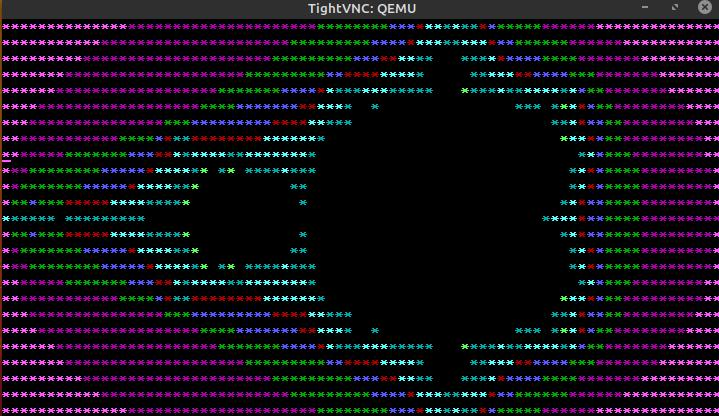
\includegraphics[scale=0.8]{figures/terminal-output.jpg}
    \caption{Rendering of the Mandelbrot set in the InfOS shell}
    \label{terminal-output}
\end{figure}

One other important point to note is that the Mandelbrot set is traditionally computed using floating point arithmetic. While InfOS does have a floating point unit, it does not routinely save and restore the floating point registers during a context switch, in order to reduce switching overhead. This means that with a multithreaded execution of the benchmark, any floating point computation would be overwritten and interfered with by other threads, unless the floating point state was saved. I did spend some time trying to save floating point state on a context switch using the \verb|xsave| instruction, but this turned out to be more complex than expected and I wasn't able to implement this within the time available. Because the focus of this project is parallel computation rather than floating point arithmetic, I instead decided to implement the Mandelbrot algorithm using fixed-point arithmetic and left the floating point context switching as future work. A fixed-point number representation simply stores all values multiplied by some normalisation factor, uses integer operations for calculations, and then normalises the result when required. By choosing the multiplier to be a power of 2, I was able to compute the Mandelbrot set using only integer operations, and then use bit shifting operations to quickly perform multiplication and division when necessary.

As already discussed, the program supported varying the number of threads alongside the number of cores, since for $x$ cores to be utilised effectively, there must be at least $x$ independent threads ready for execution. This allowed me to experiment with the following three scenarios:

\begin{enumerate}
    \item Unicore, single-threaded 
    \item Unicore, multithreaded 
    \item Multicore, multithreaded
\end{enumerate}

The unicore, single-threaded case provided a baseline to compare execution times against. It was important to separate the two multithreaded cases because even in the unicore case, multithreading alone can improve performance. For example, processor throughput can be increased by replacing a blocked thread with one that is ready to execute, until the blocked thread is ready to resume execution. If the system's threads are mostly I/O-bound, then multithreading alone can improve performance by increasing processor throughput. If, however, the threads are mostly compute-bound, then processor throughput will already be maximised and multithreading alone should have little impact. Here, we put the compute-bound theory to the test, but we were unable to test the implementation on an I/O-bound benchmark because InfOS does not currently support asynchronous I/O, and adding support would be beyond the scope of this project. However, on such a benchmark, I would expect to see a performance improvement with both the introduction of multithreading and the introduction of multicore. That is, the unicore, single-threaded case would again be the baseline, the unicore, multithreaded case would provide a performance improvement over the baseline, and the multicore, multithreaded case would likely provide a second improvement over that.

In order to determine if any performance difference was really caused by introducing additional cores, as opposed to making the Mandelbrot program multithreaded, I isolated the changes between experiments. The combinations of threads and cores used can be seen in table \ref{timing-infos-mb}, with horizontal lines separating five distinct cases: unicore and single-threaded, unicore and multithreaded, and then multithreaded with two, three and four cores respectively. For each configuration, I timed the real execution time using a timing program written in InfOS user space. This timing program was verified using an external stopwatch to ensure accuracy before experiments began. Each parameter configuration was executed three times, and then the execution times were averaged, to give the results shown in table \ref{timing-infos-mb}.

\subsection{Results} \label{mb-benchmark-results}
The baseline performance on the Mandelbrot benchmark was 9.143 seconds in the unicore, single-threaded case. The results for the unicore, multithreaded case show that introducing multithreading had very little impact on the execution time. In fact, the execution time actually increased slightly to about 9.4 seconds. This is consistent with my expectations, because the Mandelbrot program involves extensive computation and very little I/O, meaning that the threads are compute-bound. This gives no opportunity to interleave threads while other threads are waiting, so multithreading simply introduces additional overhead with no performance benefit. 


\begin{table}[h]
\begin{minipage}{.3\textwidth}
\vfill
\centering
\scriptsize
\begin{tabular}{ccc}\toprule
Cores & Threads & Average time (s) \\
\midrule
1 &1 &9.143 \\
\midrule
1 &2 &9.150 \\
1 &4 &9.400 \\
1 &8 &9.387 \\
1 &16 &9.243 \\
1 &32 &9.430 \\
\midrule
2 &2 &4.753 \\
2 &4 &4.930 \\
2 &8 &4.950 \\
2 &16 &4.887 \\
2 &32 &4.873 \\
\midrule
3 &2 &\textbf{4.900} \\
3 &4 &3.453 \\
3 &8 &3.447 \\
3 &16 &3.377 \\
3 &32 &3.390 \\
\midrule
4 &2 &\textbf{4.910} \\
4 &4 &2.647 \\
4 &8 &2.670 \\
4 &16 &2.677 \\
4 &32 &2.687 \\
\bottomrule
\end{tabular}
\captionof{table}{Average time taken in seconds for InfOS to execute the Mandelbrot benchmark with varying numbers of cores and threads}\label{timing-infos-mb}
\end{minipage}\hfill\hfill
\begin{minipage}{0.65\textwidth}
\centering
% \begin{figure}[h]
    
    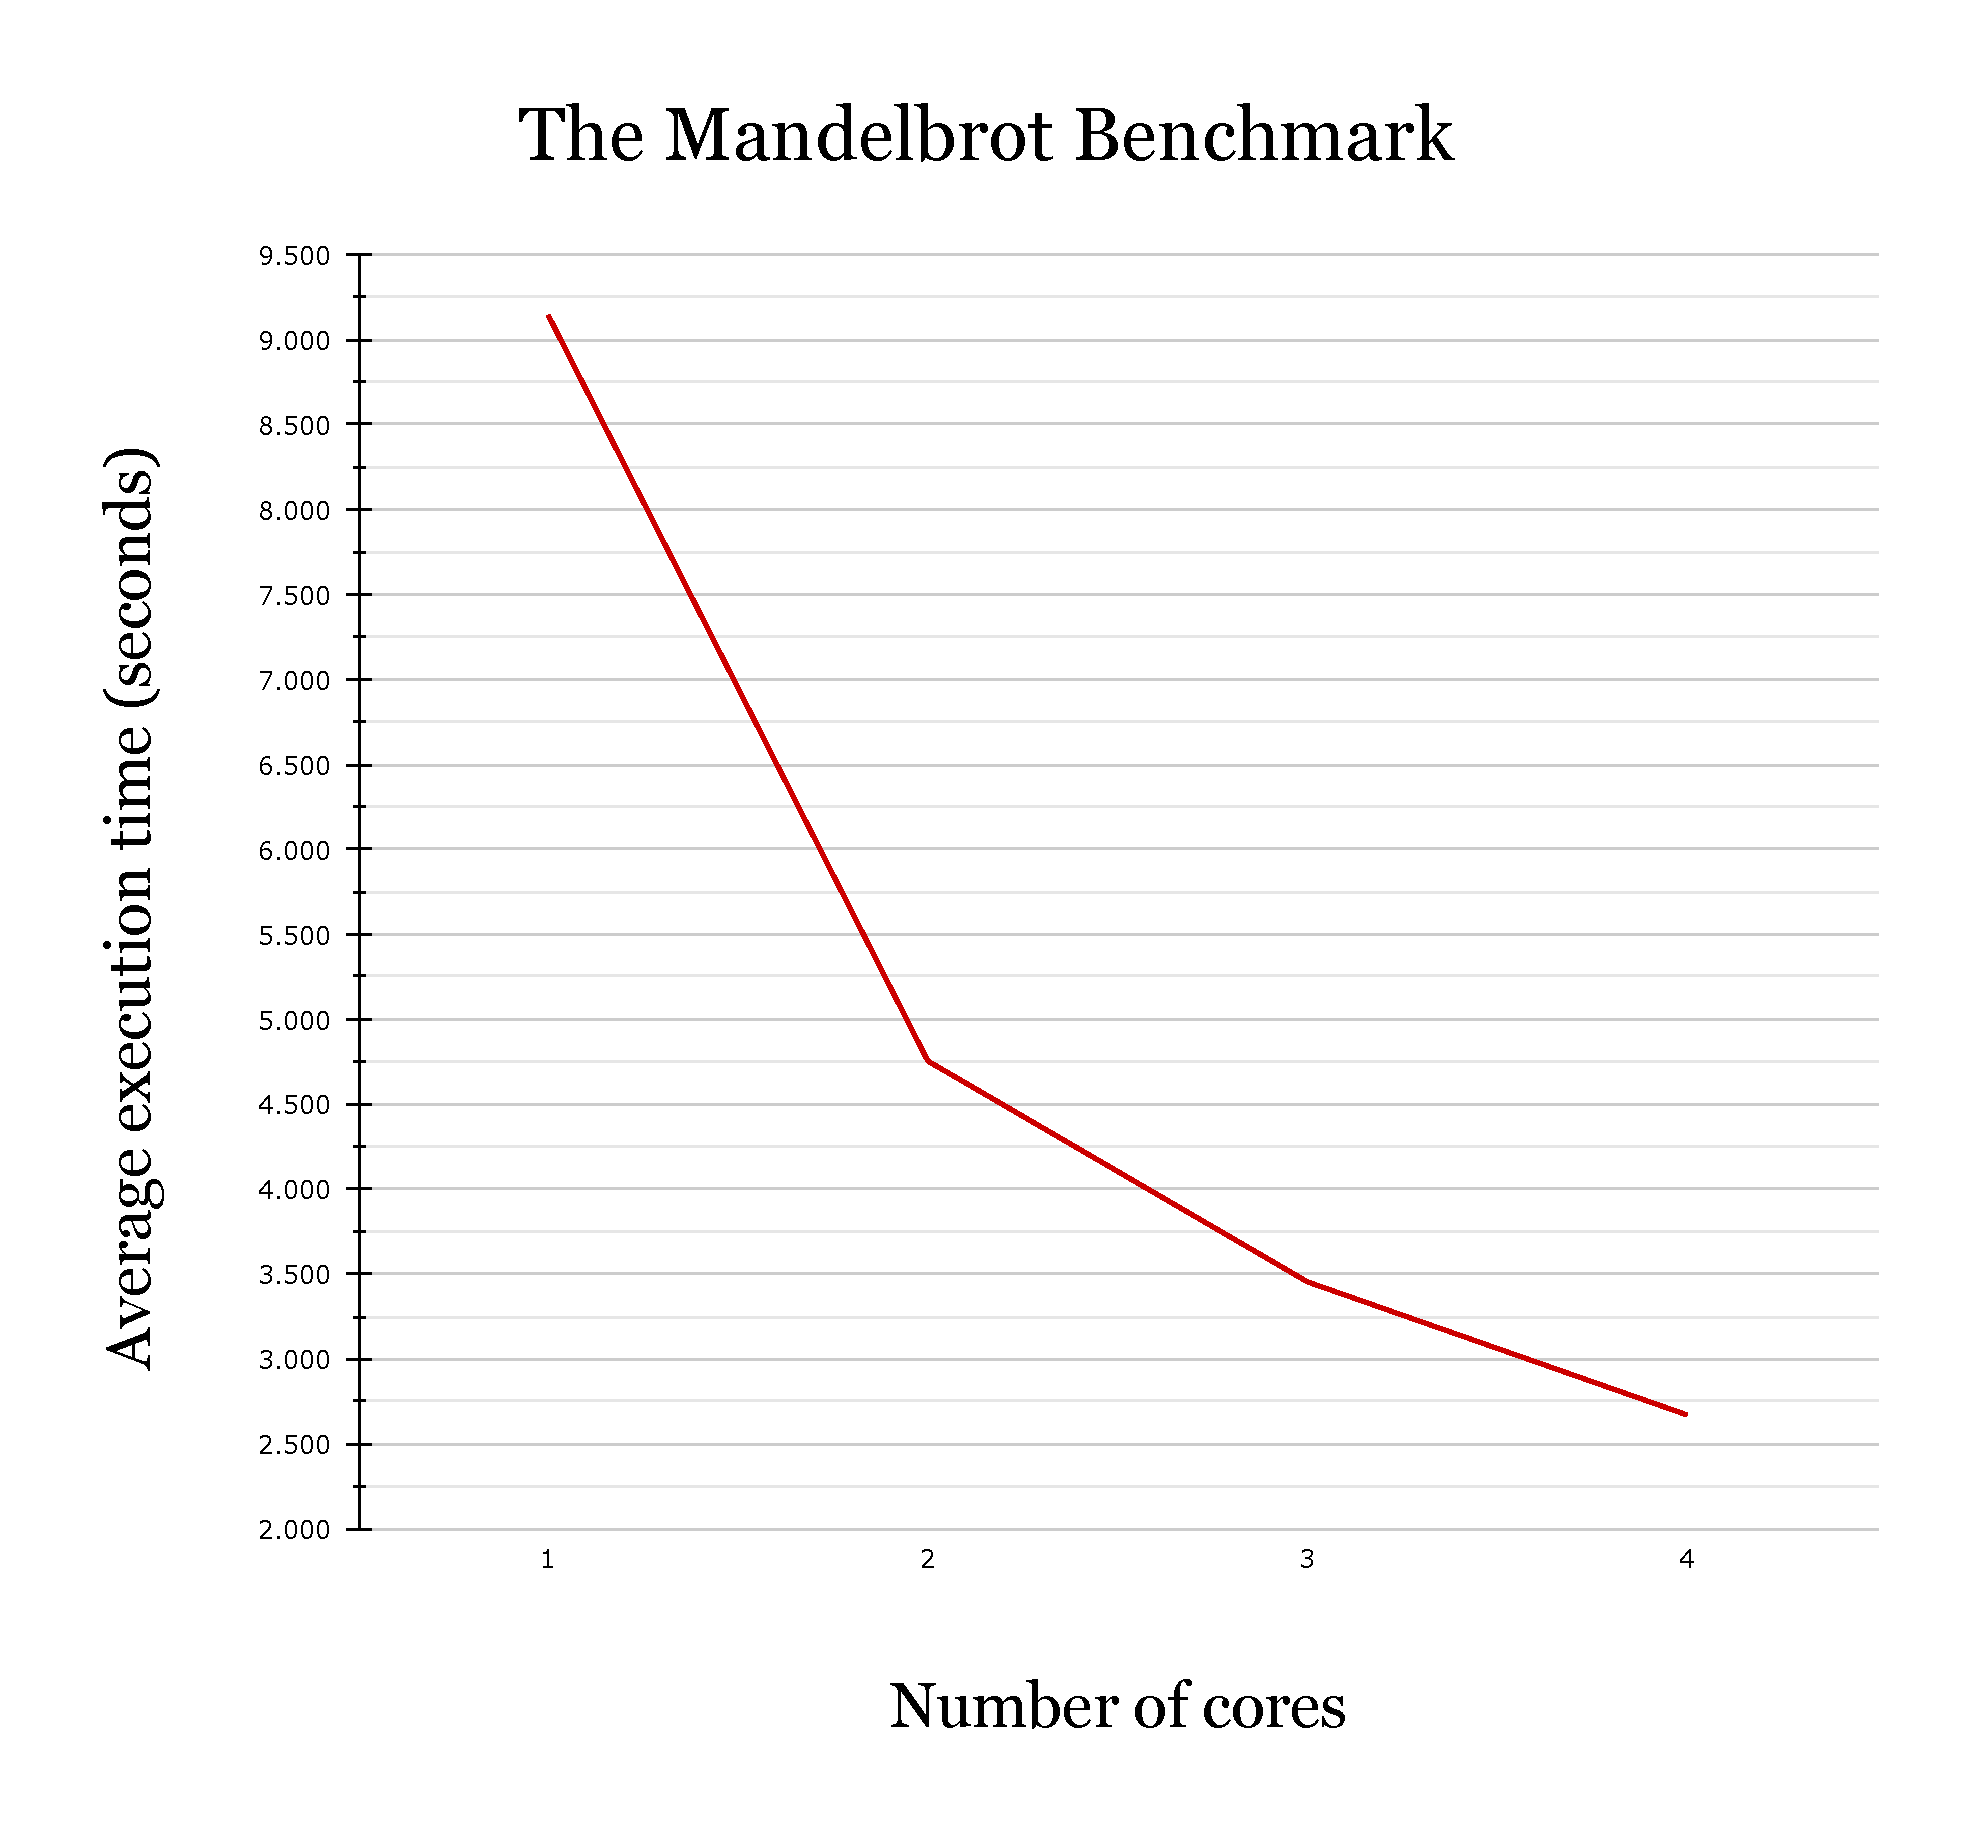
\includegraphics[scale=0.3]{figures/mandelbrot-graph.pdf}
    \captionof{figure}{Number of cores plotted against average time taken for InfOS to execute the Mandelbrot benchmark once the thread count met or exceeded the number of cores}
    \label{mandelbrot-graph}
% \end{figure}
\end{minipage}
\end{table}


In the multicore, multithreaded case, the execution time decreases with each additional core, with the exception of the two cases highlighted in bold. In the case with three cores and two threads, the thread count is not high enough to keep all cores busy. One core must be sat idle at any given point, which is why the performance is at a similar level to the dual-core case. Similarly, in the case with four cores and two threads, two cores are sat idle, and the performance is again similar to the dual-core case. Again, the results show that increasing the number of threads past the number of cores does not decrease the execution time any further, due to each core already being fully utilised by the compute-bound threads.

It is clear to see that any performance benefit gained was the result of introducing additional cores to the system. To see the trend, I plotted the number of cores against the average performance once the thread count met or exceeded the number of cores: that is, one core one thread, two cores two threads, three cores four threads and four cores four threads. This plot is shown in figure \ref{mandelbrot-graph}. Clearly, with the introduction of additional cores, the execution time decreases, but the trend is not quite linear. I was interested to learn more about how this scaling compared to how other operating systems utilise additional cores, which led me to run a second benchmark, described in section \ref{mb-mod-benchmark}.

\section{Scalability Benchmark}
\label{mb-mod-benchmark}
\subsection{Environment} 
As previously mentioned, the more cores available to InfOS, the better the performance. However, I wanted to compare this performance scaling to a highly-developed and well-established operating system in order to visualise how efficiently InfOS uses the additional available resources. To do this, I ported the Mandelbrot benchmark into a Linux version. Since the pixels may be computed out of order, the original Mandelbrot benchmark displays the output to the terminal correctly by allowing each thread to specify exactly which $(x,y)$ point to print which colour to. There is no way to do this in standard C++ without writing additional complex functionality, so the benchmark was modified to save the pixel value to a global two-dimensional array, rather than printing the value to the screen. I controlled the number of threads by creating pthreads, and I controlled the number of cores by affining those threads to a processor set: so in the unicore case, all threads were affined to a singleton processor set, in the dual-core case, all threads were affined to a processor set containing two cores, and so on.

% In order to ensure fairness, the frequency of InfOS was changed from 100Hz to 250Hz, to match Linux's value. 

I then reran the same core and thread configurations as in table \ref{mb-benchmark-results} on InfOS, but using the modified Mandelbrot benchmark. I also ran this modified Mandelbrot benchmark on Linux, again with the same core configurations as in table \ref{mb-benchmark-results}. I timed the Linux execution using the \verb|time| command, and again, verified this with an external stopwatch to ensure accuracy. I also manually set the Linux scheduler to be FIFO and gave the threads maximum priority, to ensure they had the best possible chance of executing quickly. This gave the results shown in tables \ref{timing-scalability-infos} and \ref{timing-scalability-linux}.

\begin{table}[h]
\parbox{.45\linewidth}{
\centering
\scriptsize
\begin{tabular}{ccc}
\toprule
Cores &Threads &Average (s) \\
\midrule
1 &1 &9.210 \\
\midrule
1 &2 &9.200 \\
1 &4 &9.378 \\
1 &8 &9.367 \\
1 &16 &9.135 \\
1 &32 &9.273 \\
\midrule
2 &2 &4.539 \\
2 &4 &4.736 \\
2 &8 &4.763 \\
2 &16 &4.587 \\
2 &32 &4.644 \\
\midrule
3 &2 &\textbf{4.678} \\
3 &4 &3.228 \\
3 &8 &3.260 \\
3 &16 &3.184 \\
3 &32 &3.266 \\
\midrule
4 &2 &\textbf{4.676} \\
4 &4 &2.429 \\
4 &8 &2.457 \\
4 &16 &2.473 \\
4 &32 &2.451 \\
\bottomrule
\end{tabular}
\caption{Average time taken in seconds for \textbf{InfOS} to execute the scalability benchmark with varying numbers of cores and threads}\label{timing-scalability-infos}
}
\hfill
\parbox{.45\linewidth}{
\centering
\scriptsize
\begin{tabular}{ccc}
\toprule
Cores &Threads &Average (s) \\
\midrule
1 &1 &8.937 \\
\midrule
1 &2 &8.864 \\
1 &4 &8.708 \\
1 &8 &8.857 \\
1 &16 &8.866 \\
1 &32 &8.873 \\
\midrule
2 &2 &4.584 \\
2 &4 &4.572 \\
2 &8 &4.542 \\
2 &16 &4.449 \\
2 &32 &4.466 \\
\midrule
3 &2 &\textbf{4.578} \\
3 &4 &3.079 \\
3 &8 &3.158 \\
3 &16 &3.162 \\
3 &32 &3.185 \\
\midrule
4 &2 &\textbf{4.563} \\
4 &4 &2.432 \\
4 &8 &2.382 \\
4 &16 &2.359 \\
4 &32 &2.426 \\
\bottomrule
\end{tabular}
\caption{Average time taken in seconds for \textbf{Linux} to execute the scalability benchmark with varying numbers of cores and threads}\label{timing-scalability-linux}
}
\end{table}

\subsection{Results}

The InfOS execution times were very similar to the previous benchmark, confirming that the minor functionality changes did not alter the program's behaviour. Making a direct comparison between the results obtained on this benchmark, the Linux execution times were very similar to the InfOS execution times. The operating systems both showed almost identical behaviour to that observed in the previous section, namely:

\begin{enumerate}
    \item Multithreading in the unicore case did not impact execution time.
    \item In the case where there were less threads than cores, performance was negatively affected by one or more cores being idle.
    \item Increasing the number of threads past the number of cores made little further difference to performance.
    \item With every additional core, the execution time decreased.
\end{enumerate}

To compare the resource utilisation, we can look at the number of cores against the average performance once the thread count met or exceeded the number of cores for each operating system. This data is extracted and shown in table \ref{timing-scalability-abridged}. From this data, we can calculate the percentage performance increase gained with each additional core relative to the performance without the additional core. That is, we compute the percentage performance increase for two cores relative to the unicore case, with three cores relative to the dual-core case, and so on. These percentages can be seen in table \ref{timing-scalability-percentages}, and figure \ref{scalability-graph} shows this data graphically. We can see that the trend of performance against additional resources is about the same for both InfOS and Linux. That is, when given additional resources, InfOS is able to extract the same performance benefit from them that Linux can, confirming that the multicore implementation accurately represents the way a real operating system handles multiple cores.

\begin{table}[h]
\parbox{.45\linewidth}{
\centering
\scriptsize
\begin{tabular}{cccc}\toprule
Cores & Threads & InfOS & Linux \\
& & average & average \\
& & time (s) & time (s) \\
\midrule
1 & 1 & 9.210 & 8.937 \\
\midrule
2 & 2 & 4.539 & 4.584 \\
\midrule
3 & 4 & 3.228 & 3.079 \\
\midrule
4 & 4 & 2.429 & 2.432 \\
\bottomrule
\end{tabular}
\caption{Average time taken in seconds for InfOS and Linux to execute the scalability benchmark once the thread count met or exceeded the number of cores}\label{timing-scalability-abridged}
}
\hfill
\parbox{.45\linewidth}{
\centering
\scriptsize
\begin{tabular}{cccc}\toprule
Cores & Threads & InfOS & Linux \\
& & performance & performance \\
& & increase & increase \\
\midrule
2 & 2 & 50.72\% & 48.71\% \\
\midrule
3 & 4 & 28.88\% & 32.83\% \\
\midrule
4 & 4 & 24.75\% & 21.01\% \\
\bottomrule
\end{tabular}
\caption{Performance increase with every additional core relative to performance immediately prior to adding that core}\label{timing-scalability-percentages}
}
\end{table}

\begin{figure}[h]
    \centering
    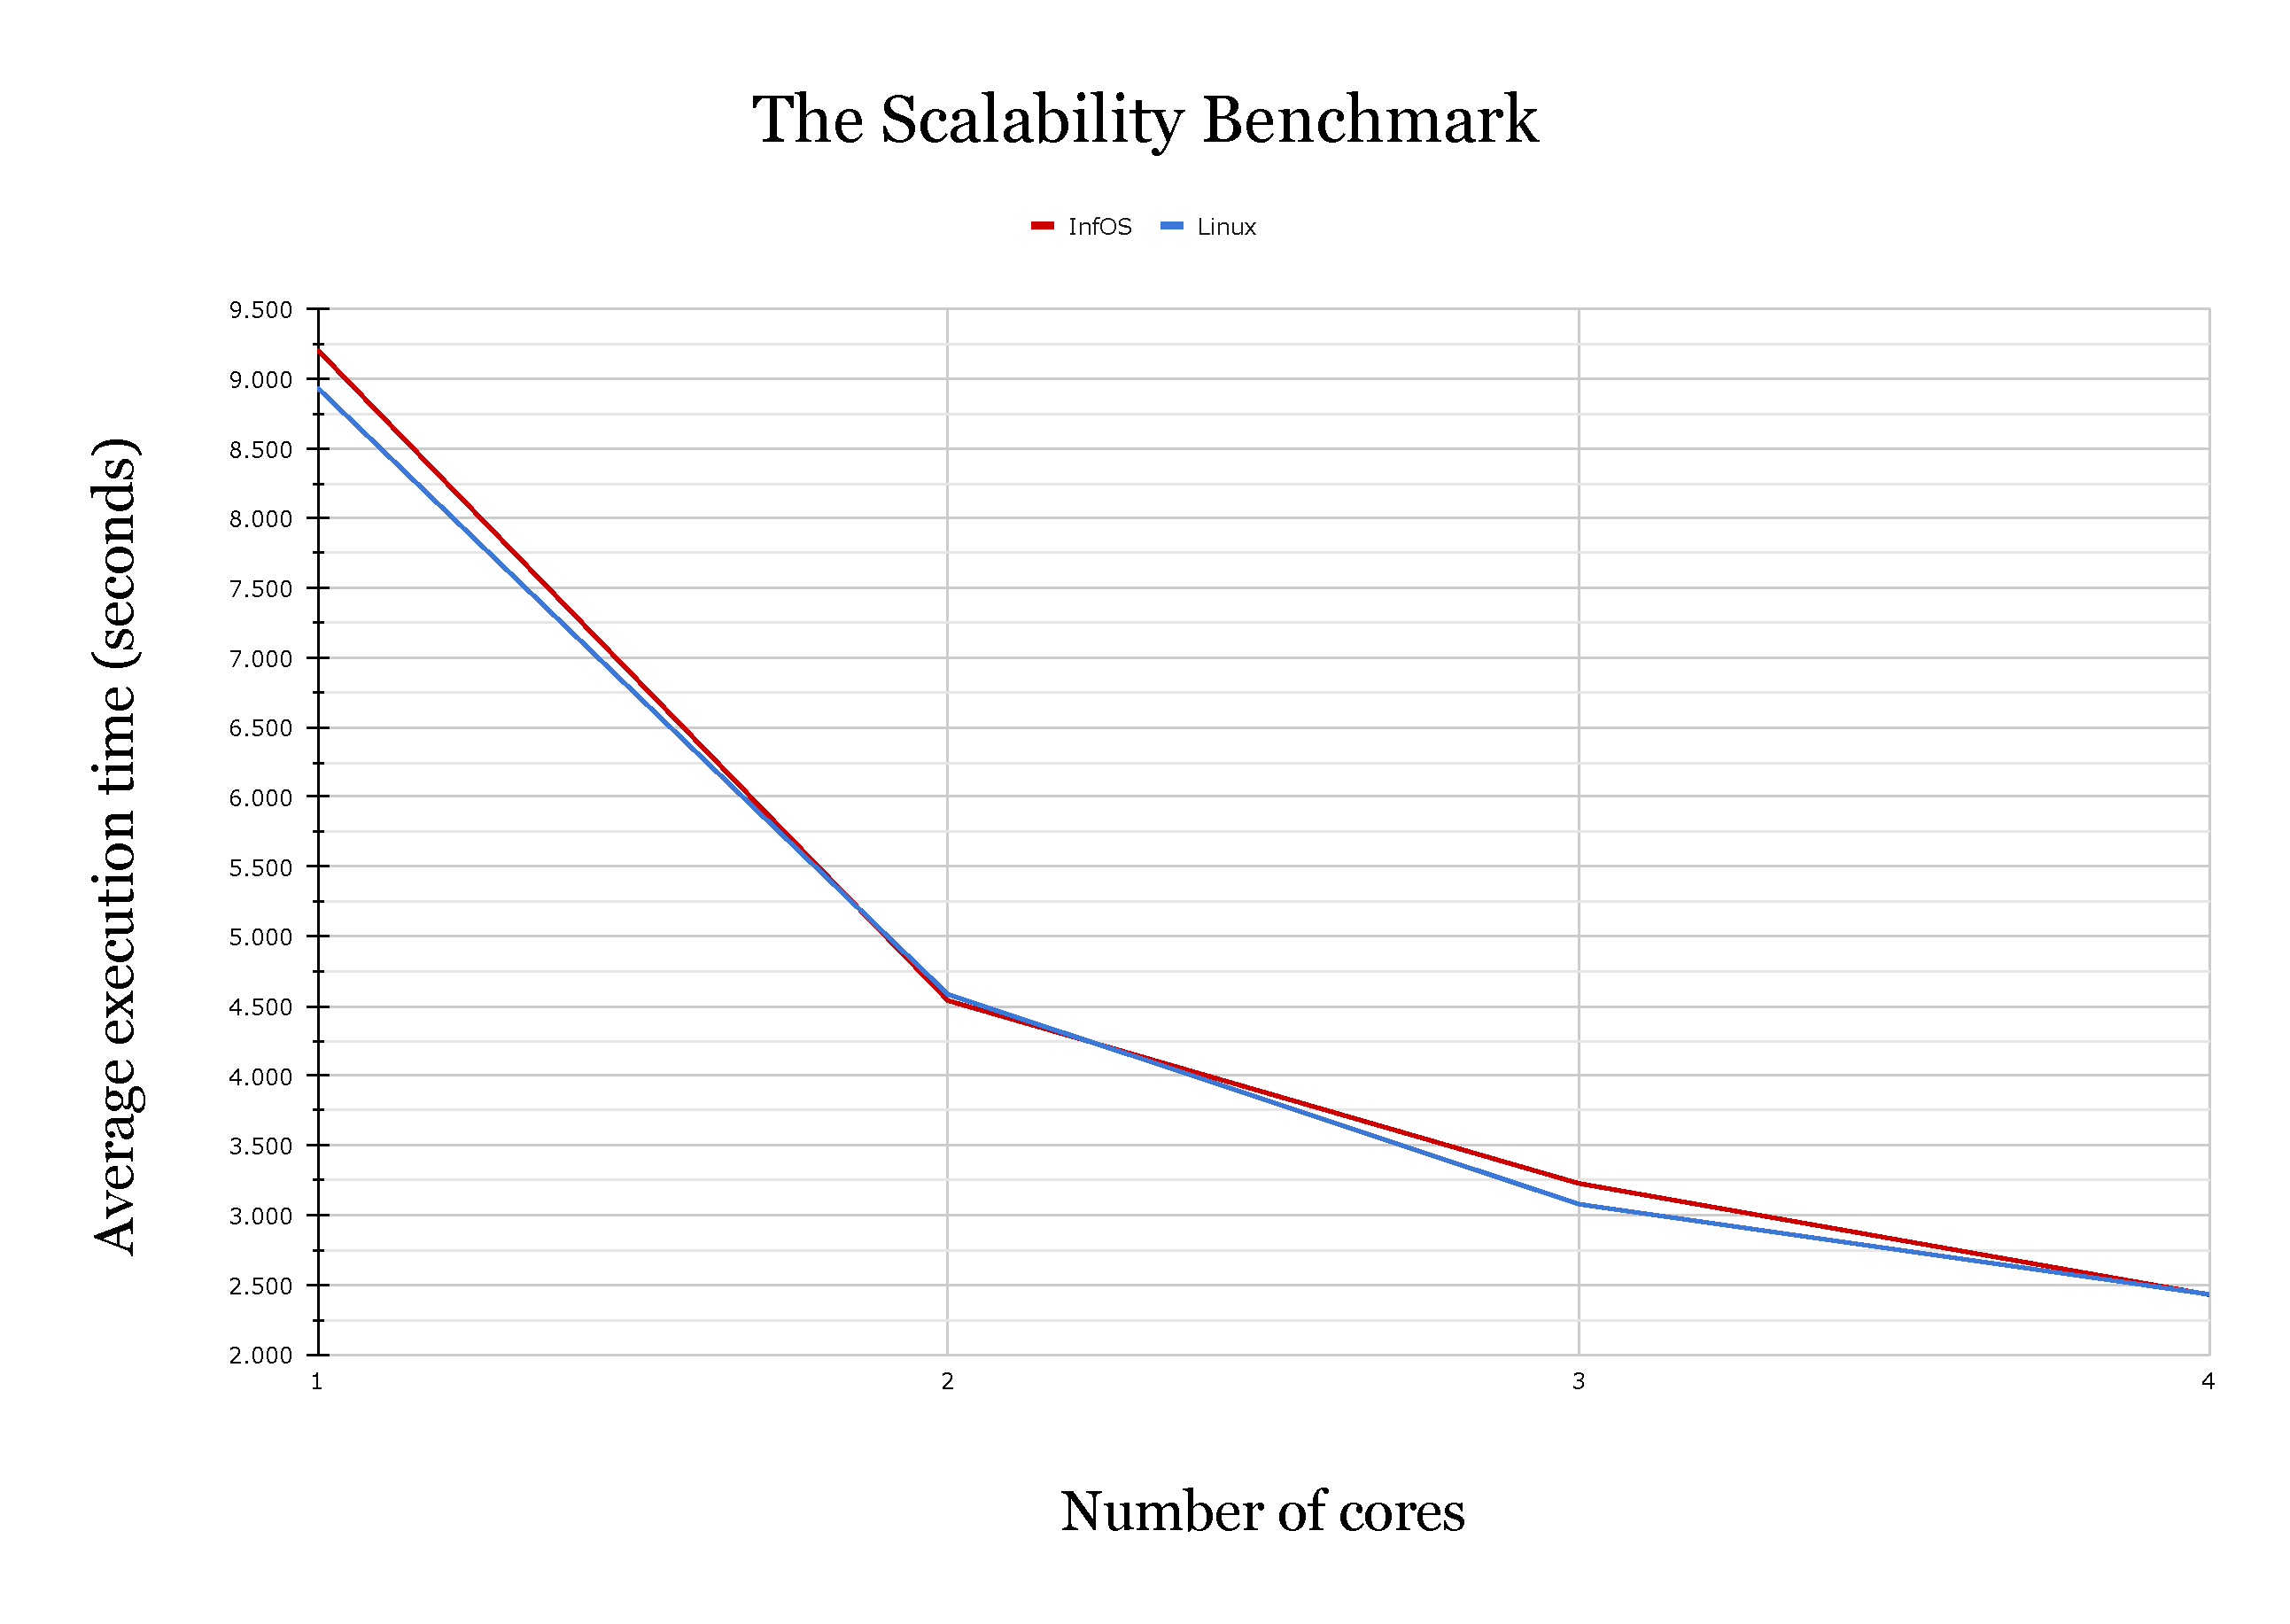
\includegraphics[scale=0.3]{figures/scalability-graph.pdf}
    \caption{Number of cores plotted against average time taken for InfOS and Linux to execute the scalability benchmark once the thread count met or exceeded the number of cores}
    \label{scalability-graph}
\end{figure}

\chapter{Conclusion}
\section{Discussion}
This project provides three key contributions, as discussed in section \ref{key-contributions}:
\begin{description}
    \item [Teaching contributions.] A well-designed, object-oriented multicore operating system that can be easily understood by students.
    \item [Technical contributions.] AA working operating system implementation that can be downloaded and booted on real hardware by anyone.
    \item [Research contributions. ] A platform on which to build further research and experiment with performance optimisations.
\end{description}

\subsection{Teaching Contributions}
As with the rest of InfOS, the multicore implementation was designed specifically with structure and readability in mind. The original boot code was a series of initialisation function calls for different subsystems. For example, \verb|mm_init| initialises the memory management subsystem, before \verb|acpi_init| parses the ACPI tables. I extended this, defining a function \verb|cpu_init| and calling that from the original boot code. This makes it clear for students to see at what point the multicore initialisation is done during the operating system boot process.

The C++ language's object-oriented support provided flexibility when modelling the cores. As discussed in section \ref{implementation}, the cores, LAPICs, LAPICTimers, schedulers and scheduling manager are all modelled as subclasses of the device object. The global device manager object provides centralised access to all other devices in the system, and devices communicate by calling methods on other device objects. For example, cores send IPIs by calling the \verb|send_remote_sipi| function defined within the LAPIC class on their LAPIC instance. Recall from section \ref{initialising-cores} that within \verb|cpu_init|, the function \verb|start_core| contains the general procedure for waking each core. This is called on every core object in the system, making the generic waking code simple to understand. Also recall from section \ref{calibrating-timers} that all calibration code is defined within the core class, in methods such as \verb|lapic_init| and \verb|timer_init|, making the AP calibration code itself very short and readable: simply a series of calls on the AP object to these initialisation functions. This modular structure makes the entire multicore initialisation control flow path very easy to follow throughout the system.

InfOS also models processes and threads as distinct objects, as opposed to Linux's implementation, which doesn't differentiate between the two. Within InfOS, processes have a private address space and one or more threads, whereas threads have an associated context but share the address space of their process parent. This makes the conceptual difference between processes and threads explicit, aiding students in learning the core theoretical concepts, which can then be generalised to other operating system implementations. Recall that the scheduler works with scheduling entity objects, which are currently threads. However, section \ref{scheduling-threads} noted that processes could easily extend the scheduling entity class, allowing the programmer to change InfOS's unit of work from threads to processes, or perhaps both. This separation of the concepts again helps the student to understand the underlying theory, without being too focused on one specific operating system implementation. The design choices discussed have not been detrimental to performance either, as evidenced by the scalability comparison in section \ref{mb-mod-benchmark}: InfOS achieves the same percentage performance improvement with additional cores as Linux does. This project has therefore achieved the goal of producing a teaching operating system with simple, readable, modular code, that still accurately represents the behaviour of larger operating systems.

\subsection{Technical Contributions}
The multicore implementation will be made open-source and merged into the public InfOS GitHub repository \cite{infos}. It will be used for the next iteration of the UG3 Operating Systems course, and it is also freely accessible to the public. It is available to view, modify and run, either in an emulator like QEMU \cite{qemu}, or on real hardware by booting from a USB drive, achieving the technical contribution.

\subsection{Research Contributions}
The scalability comparison in section \ref{mb-mod-benchmark} confirms that the multicore implementation is utilising the cores in a sensible way, but we do not see the near-linear trend that the literature review in section \ref{towards-multicore} suggested was possible. InfOS handles load balancing in a similar way to Linux; however, the literature suggests that Linux's approach to load balancing is sub-optimal, with one study noting several performance bugs that lead to cores sitting idle \cite{wasted-cores}. Recall that the authors of the study suggested that  while ongoing research has discovered promising scheduling algorithms, the monolithic nature of operating system schedulers like Linux's make these algorithms impractical to implement and test without adding significant complexity. The authors suggested that a modular scheduler would allow further research into how different load balancing approaches can be combined to suit different system workloads \cite{wasted-cores}.

InfOS can provide this functionality. While Linux's scheduler is modular in the sense that it allows selection between different scheduling policies such as first-in-first-out or round-robin, it has a monolithic load balancing policy applied uniformly to all tasks and cores in the system. InfOS takes this a step further, allowing both modular selection of the scheduling policy, and also modular selection of the load balancing algorithm, providing flexibility for different workloads. This gives the perfect opportunity for further research into scheduling algorithms that effectively utilise all available processing resources. We discuss further in section \ref{future-work} how we are using InfOS as a platform for future research.


% To make the difference clear, consider a system with two cores running three threads: T1 and T2 on core 1, and T3 on core 2. If the scheduling policy was set to round-robin at boot time, the cores would schedule their own threads according to that policy, so core 1 would execute T1, T2, T1, T2 and so on, and core 2 would execute T3 only. If another thread, T4, were to be created, the global scheduling manager may now choose to dispatch T4 to either core 1 or core 2. Dispatching T4 to core 2 may seem like the natural choice to keep the workload balanced, but if T4 had previously been executing on core 1 and had data cached there, the performance benefit gained by using the warm cache may outweigh the imbalanced workload. Here, we are interested in the distribution decisions made by the global scheduling manager and their impact on performance, but \textbf{not} in the scheduling policies used by the individual cores. For the avoidance of doubt, I will refer to the former as ``load balancing policy", and the latter as ``scheduling policy". 

\section{Future Work} \label{future-work}
A number of factors affect how the operating system's workload should be distributed, including the available resources, the number of threads and the nature of those threads (I/O-bound or compute-bound). The behaviour of threads also changes over time, and this dynamic nature means that an adaptive load balancing approach may be more practical than a static one \cite{adaptive-sched}. For example, with programs involving repeated data accesses, the load balancing approach should prioritise keeping threads executing on their affined cores where possible. However, for a workload with a mixture of I/O-bound threads and compute-bound threads, the thread nature may be a more important consideration. Consider a system with four threads: two I/O-bound threads, and two compute-bound threads. A simple load balancing approach may consider the following situation well-balanced: both of the I/O-bound threads on one core and both of the compute-bound threads on the other core. However, the I/O-bound thread core could be regularly sat idle with both threads blocked, while the compute-bound thread core could be overwhelmed with both threads demanding processor cycles. Migrating the threads to evenly distribute the work might be beneficial, even if this results in an initial cache flush. Introducing thread priority levels would further complicate the matter. 

Furthermore, the memory access patterns of threads may conflict with one another, meaning that threads may regularly evict cache lines belonging to other threads, increasing miss rates. Intuitively, these threads should not be allocated to the same core if possible, and recent research suggests that intelligent scheduling approaches could not just consider which cache a thread has warmed to, but also that particular cache's statistics. A recent study has proposed a multi-metric scoring scheme that allows the scheduler to consider a thread's execution characteristics \cite{adaptive-sched}. Another study considers contention for other shared resources in addition to the cache, such as the memory controller, the memory bus and prefetching hardware. A scheduling algorithm considering these resources was demonstrated to perform within 2\% of the optimal \cite{contention-aware-sched}. Clearly, there are many factors that the scheduler may take into account when trying to find the optimal way to schedule threads. There is plenty of scope for further research into this area, and we are working on a research paper investigating intelligent, cache-aware scheduling policies and integrating them into InfOS to evaluate performance on a real operating system. Section \ref{load-balancing-policies} describes the research that is currently underway.


% For example, if two threads were sharing a core and were accessing the same cache lines, they would continually evict one another's data. While migrating one thread would initially result in a cache flush, the performance benefits could then be regained once the thread has warmed to its new core and is no longer having data evicted regularly.


\subsection{Load Balancing Policies} \label{load-balancing-policies}
As a proof-of-concept, I added another command line parameter to select the load balancing policy and wrote the implementations for the random and round robin policies. Future work would involve extending this interface by adding implementations for the remainder of the policies to allow running the experiments and drawing comparisons.

\begin{description}
\item[Random.] Uses the \verb|rdrand| instruction to read a random value and takes this number modulo the number of cores available to the system. Uses this number as an index into the list of cores available.
\item[Round robin.] Removes a core from the head of the list and appends it to the end of the list. Returns this core as the one to dispatch the task to.
\item[Load balancing.] Chooses the core with the smallest workload. There are many possible definitions of `load' to consider here.
\item[Processor affinity.] Tries to reduce cache flushes by allocating threads back to the core on which they were recently running.
\item[Cache-aware.] Considers statistics such as cache misses and tries to allocate threads to cores in a way that reduces cache contention.
\end{description}

\subsection{Benchmark}
To put these policies to the test, they need to be executed on a system with a dynamic workload, otherwise the load balancing task is fairly simple. For example, an asynchronous workload would have thread sleeping and waking frequently, prompting the scheduling manager to continually try to balance the load. If the scheduling manager is migrating the threads between cores a lot, recall that this will result in cache flushes, which may be detrimental to performance. A good benchmark would therefore be a program involving lots of asynchronous events and lots of cache accesses. I wrote a benchmark loosely inspired by the Bitcoin proof-of-work algorithm \cite{proof-of-work}, which has a global integer array and a number of threads. Each thread is allocated one section of the array and must repeatedly compute the hash of this section, where the hash is essentially the sum of the elements in the section with some salt value. The salt is incremented on every iteration, which increases the sum until the hash exceeds a certain value. Dividing the array between the threads and requiring repeated calculation of the sum means that each thread is repeatedly accessing the same data, which would benefit from being in the core's private cache. In order to simulate blocking for I/O or waiting for some other event, after each calculation, the thread sleeps for a random amount of time, generated using the \verb|rdrand| function. When each thread awakes, it returns to the global scheduling manager, who then decides which core to dispatch the task to. This benchmark means that each thread is essentially accessing the same data repeatedly, but potentially migrating between cores and suffering cache flushes. A future experiment could then take the policies defined in section \ref{load-balancing-policies} and evaluate them on the above benchmark to evaluate the impact of different workload management on performance.

\bibliographystyle{plain}
\bibliography{mybibfile}

\end{document}
